%% Ez a fájl felelős azért, hogy beállítsa, hogy hogyan nézzen ki a dokumentum, leírja az összes formázást. A fájl végén található rész pedig elindítja a pdf generálását a contents.tex importálásával.

% Általános formázások
% -------------------------------------------------------

% twoside: kétoldalas nyomtatás --> írd át oneside-ra, ha egyoldalasan nyomtatod (de ne nyomtasd egyoldalasan, mert a TVSZ is kétoldalas nyomtatást javasol)
% 11pt: betűméret
\documentclass[a4paper,11pt,oneside]{report}

% Betűtípus váltása
%\renewcommand{\familydefault}{ppl}
% További betűtípusok: https://www.sharelatex.com/learn/Font_typefaces

% Tartalomjegyzék formázásához
\usepackage{tocloft}
% Tartalomjegyzékben az al-alfejezetek (\section) indentálása
\setlength{\cftsecindent}{.9cm}
% Tartalomjegyzékben az al-alfejezetek (\subsection) indentálása
\setlength{\cftsubsecindent}{1.4cm}

% Ezzel ha két bekezdés közé üres sort teszel, akkor a kimeneti pdf-ben is megjelenik térköz a két bekezdés közt
%\usepackage{parskip}
% -------------------------------------------------------


% Fejezetcímek formázása
% -------------------------------------------------------
\usepackage{titlesec}

% Milyen mélységig legyenek számozva az fejezetek
% 0: csak a fejezetek (\chapter) vannak számozva (bevezetés, irodalomkutatás stb.)
% 1: alfejezetek (\section) is számozva vannak
% 2: al-alfejezetek (\subsection) is számozva vannak
\setcounter{secnumdepth}{2} 

% Fejezetcímek formázása
% Közvetlenül a fejezetcím előtt legyen a szám, "fejezet" szó pedig nem kell.
\newcommand{\titleformatting}{
    %\titleformat{\chapter}{\normalfont\huge}{\thechapter.}{1em}{\huge\textbf}
}

% Az alfejezet-címek (\section) száma előtt ne szerepeljen a fejezet (\chapter) száma (pl 2.1 helyett csak simán 1)
%\renewcommand\thesection{\arabic{section}}

% Alfejezetcímek formázása:
%\titleformat{melyik elem}[block/wrap]{számozás formázásai}{számozás maga}{térköz a számozás és a cím között}{cím formázásai}
% méretek: \large, \Large, \huge, \Huge
% további formázási lehetőségek: \bfseries (vastag), \it (dőlt), \underline (aláhúzott)
% \thesection: Az adott cím sorszámát helyettesíti be (épp ezért kell a pont a \thesection parancs után, hogy a cím sorszáma után legyen pont)
\titleformat{\section}[block] {\normalfont\Large\bfseries}{\thesection.}{1em}{\Large}
% -------------------------------------------------------


% Kötelező formázás
% -------------------------------------------------------

% margók
\usepackage[margin=2.5cm, bindingoffset=1.25cm]{geometry}

% másfeles sorköz
% \usepackage[onehalfspacing]{setspace}
\linespread{1.5}
% -------------------------------------------------------


% Hasznos csomagok
% -------------------------------------------------------

% ékezetes betűk kezelése
\usepackage[utf8]{inputenc}

% ékezetes betűknél is legyen automatikus elválasztás
\usepackage[T1]{fontenc}

% nyelvi csomag
\usepackage[english]{babel}

% képletekhez kell
\usepackage{mathtools}                        

% bibliográfia (IEEE formátumban)
\usepackage[style=ieee, backend=biber]{biblatex}

% ez az ITK logó pozicionálásához kell
\usepackage[export]{adjustbox}

% kattintható tartalomjegyzék és hivatkozások
\usepackage[hidelinks, unicode, pdfusetitle]{hyperref}
\usepackage{cleveref}
\crefname{lstlisting}{code}{code}
\Crefname{lstlisting}{Code}{Code}

% PDF könyvjelzők
\usepackage{bookmark}

% Színes cellák táblázatokban
\usepackage[table,xcdraw]{xcolor}

% Hyperlinks - URL-ek a szövegben
\usepackage{url}

% Hosszabb idézetek
\usepackage{csquotes}
\usepackage{multicol}

\usepackage{pdfpages}
\usepackage{rotating}

% a bibliográfiában megfelelően legyenek formázva az idézőjelek
\DeclareQuoteAlias{german}{magyar}

% Kódrészletek
\usepackage{listings}
\usepackage{sourcecodepro} % egy jó betűtípus
\lstset{captionpos=b, numberbychapter=false, basicstyle=\ttfamily, showstringspaces=false, columns=fullflexible}

% Flow chart 
\usepackage{tikz}
\usetikzlibrary{shapes.multipart}
\usetikzlibrary{shapes.geometric, arrows}
\tikzstyle{startstop} = [rectangle, rounded corners, minimum width=3cm, minimum height=1cm, text centered, draw=black, fill=red!30]
\tikzstyle{io} = [trapezium, trapezium left angle=70, trapezium left angle=110, minimum width=3cm, minimum height=1cm, text centered, draw=black, fill=blue!30]
\tikzstyle{process} = [rectangle, minimum width=3cm, minimum height=1cm, text centered, draw=black, fill=orange!30]
\tikzstyle{decision} = [diamond, minimum width=3cm, minimum height=1cm, text centered, draw=black, fill=green!30]
\tikzstyle{arrow} = [thick,->,>=stealth]

% Kódrészletek magyar stílusú számozása
\renewcommand\lstlistingname{Code}
\makeatletter
\renewcommand\fnum@lstlisting{\lstlistingname~\ifx\lst@@caption\@empty\else\thelstlisting\fi}%
\makeatother

% Képek beszúrásakor automatikusan ebben a mappában fogja a képeket keresni
\graphicspath{ {images/} }

% Hivatkozásokat tartalmazó fájl
% \addbibresource{hivatkozasok.bib}
\addbibresource{bibliography/pynq.bib}
\addbibresource{bibliography/airsim.bib}
\addbibresource{bibliography/articles.bib}
\addbibresource{bibliography/devices.bib}
\addbibresource{bibliography/avoid.bib}
\addbibresource{bibliography/software.bib}
\addbibresource{bibliography/company.bib}
\addbibresource{bibliography/images.bib}

% Random szövegek generálása - nyugodtan töröld
\usepackage{lipsum}

% Csak hogy ne sírjon amiatt, hogy a BibLatex 3.12-es verziója rengeteg változtatást tartalmaz az előző verzióhoz képest
\BiblatexHungarianWarningOff
% Ez meg egy másik felesleges warning-ot némít el (https://tex.stackexchange.com/a/451193)
\usepackage{silence}
\WarningFilter{biblatex}{File 'english-ieee.lbx'}
% -------------------------------------------------------


% Címoldal + üres lap utána
% -------------------------------------------------------
\author{\nev\\\kepzes}
\title{\Huge{\tipus}\\[1cm]
    \huge{\cim}}
\date{\the\year}

\newcommand{\cimlap}{
    
\includegraphics[valign=m, width=50pt]{ITK_logo} \parbox[c]{0.8\textwidth}{
    Pázmány Péter Catholic University,\\
    Faculty of Information Technology and Bionics}
    \vspace*{\fill}
    
    {\let\newpage\relax\maketitle}
    \vspace*{\fill}
    \begin{center}
    \bigskip
    
    \temavezetok
    \end{center}
}

\newcommand{\ureslap}{
    \begingroup
        \pagestyle{empty}
        \cleardoublepage
    \endgroup
    \clearpage
}

\usepackage{xcolor,soul}
\sethlcolor{lightgray}
\newcommand{\codeword}[1]{
\texttt{\hl{#1}}
}
% -------------------------------------------------------


% ------------- Dokumentum legenerálása -----------------
\begin{document}

\titleformatting

% Ez a fájl felelős azért, hogy a projekt fájljait összefűzze egy kimeneti pdf-fé.

% Ezeket írd át...
\def\tipus{DIPLOMA THESIS} % --> ha MSc-s vagy, írd át "DIPLOMAMUNKA"-ra!
\def\nev{Kóta Fülöp}
\def\kepzes{Computer Science engineer MSc}
\def\cim{Development of an embedded image processor architecture on FPGAs}
\def\temavezetok{Supervisors: Dr.\ Nagy Zoltán, Dr.\ Zsedrovits Tamás}

% címlap generálása
\cimlap

% A kötelező részeket római oldalszámozással tünteti fel a tartalomjegyzékben. Ha nagy betűvel írod a "Roman"-t, akkor nagy római számokkal fog számozni.
\pagenumbering{roman}

% Kötelező részek
% Ha nem szeretnéd ezeket a részeket feltüntetni a tartalomjegyzékben, akkor egyszerűen töröld az \addcontentsline kezdetű sorokat.
% \addcontentsline{toc}{chapter}{Témabejelentő}

% Hogy kétoldalas nyomtatás esetén a témabejelentő közvetlenül a címlap után lehessen
% \ureslap

% A kétoldalas témabejelentő miatt a nyilatkozat oldalszáma 3
\setcounter{page}{3}

\addcontentsline{toc}{chapter}{Statement} 
% Itt nincs semmi teendőd

\chapter*{Statement}
I, the undersigned Fülöp Kóta, student of the Pázmány Péter Catholic University, Faculty of Information Technology and Bionics, declare that I have written this diploma thesis solely myself, without any unauthorized help, and I have only used the sources referenced. Every part quoted word by word or in a paraphrased manner is indicated clearly, with a reference made. I have not submitted this diploma thesis in any other training program.

% Aláírás sor
\begin{flushright}
	\vspace*{.5cm}\par\noindent\makebox[2.5in]{\hrulefill}
	\par\noindent\makebox[2.5in][c]{\nev}
\end{flushright}

\clearpage
\addcontentsline{toc}{chapter}{Kivonat}
\chapter*{Kivonat}
A széleskörben terjedő pilóta nélküli repülőgépek (Unmanned Aerial Vehicles UAV) növelik a a balesetek lehetőségét, ezért elengedhetetlen új módszerek fejlesztése, amik segítenek elkerülni a veszélyes közelségeket illetve baleseteket.
A repülőgépek kicsi mérete miatt csak passzív képfeldolgozó rendszerek telepítése lehetséges, azonban nagyfelbontású kamerák szükségesek egy veszélyes helyzet megfelelő távolból történő érzékelésére.
A nagy felbontású képfolyam valós idejű feldolgozására nagy számítási teljesítmény szükséges.
Ez csak alkalmazás-specifikus képfeldolgozó architektúrával lehet elérni.

Ilyen architektúrák azonban mind méretben mind energiaszükségletben túlméretesek a repülőgépekhez képest.
A megoldást a programozható logiaki áramkörök jelenthetik.
Beágyazott rendszerek mind energiafelhasználásban, mind méretben sokkal kisebbek mint a hagyományos architektúrák, ugyanakkor a probléma-specifikus algoritmus megvalósításnak köszönhetően a számítási teljesítmény nem csökken.
A beágyazott rendszerek továbbá könnyen kiegészíthetőek más hasonló rendszerekkel, hogy együtt dolgozva a számítási feladatokat megosszák egymással.

Programozható logikai áramkörök segítségével a képfeldolgozó algoritmusokat hardware szinten lehet implementálni.
Az algoritmus többi része a chipen található processzor alrendszeren tud futni, ezzel még inkább csökkentve az energiafelhasználást.

A végeredmény egy olyan hardware design ami képes feldolgozni egy $3840 \times 2160$ felbontású képet 0.04160763 másodperc alatt.
Ez a kép lehet egy UHD kamera képe nagyon részletes felbontással, de állhat 4 különálló HD kamera képéből is.
A négy kamerás megoldásnál a széles látószög lehetővé teszi a drón teljes $360^\circ$ környezetének a megfigyelését.
A rendszer mindezek mellett képes a fogyasztását 4 W alatt tartani.


\addcontentsline{toc}{chapter}{Abstract}
\chapter*{Abstract}
\paragraph{}
The widespread use of unmanned aerial vehicles (UAV) increases the risk of accidents, therefore new procedures must be developed to avoid dangerous approaches and collisions.
Due to the size of small UAVs only passive image processing systems can be used.
However, high-resolution cameras are required to detect dangerous aircraft from a large distance.
High computing performance is required to process real-time image streams arriving from the cameras, which can only be achieved quickly and efficiently by using application-specific image processing architectures.

Such architectures are too large for a UAV both in energy requirement, and size.
One possible solution is to use programmable logic circuits.
The embedded systems are smaller in size and have lower energy consumption compared to the traditional architectures, and its computing performance can be the same due to the application-specific algorithm. 
An embedded system can be also improved by adding other functions, dividing the computational tasks and further extending the possible application areas.

With Programmable Logic, the image processing tasks can be executed on hardware.
The other parts of the algorithm use the integrated processor architecture of the chip.
This approach limits the power consumption even more.

The final product is a hardware design which can process a $3840 \times 2160$ image in 0.04160763 seconds.
This image can either be one UHD camera or can be assembled from 4 different HD camera input.
With 4 wide-angle camera, the whole $360^\circ$ area of the drone can be detected.
The system in the process consumed less than 4 W of energy.

\clearpage
%% Vedd ki a százalék-jelet a következő két sor elől, ha szeretnél köszönetnyilvánítást beleírni a szakdogádba/diplomamunkádba.

% Tartalomjegyzék legenerálása
\tableofcontents 

% Az innentől következő részek arab számozással kerülnek feltüntetésre a tartalomjegyzékben
\pagenumbering{arabic}

% Tartalmi részek - módosítsd nyugodtan
\chapter{Introduction} % 10316 characters

\section{Overview of the thesis} % 846 characters
\paragraph{\Cref{ch:ant}: \nameref{ch:ant}}
The development begins with a review of the algorithm.
For this, the original developers were to great help.
The system specifications were made and the details were discussed about the exact hardware and parts.
In this chapter, the previous works are presented, and the system is introduced.

\paragraph{\Cref{ch:plan}: \nameref{ch:plan}} 
This chapter describes the work that is done with all the errors and dead ends.
The desired hardware had some issue, and change through the project, as well as the software part.
Lots of possible solutions are raced to each other, considering both development cost and applicability.
There is also the ever-changing market of image processing.
The development tools were changed during the project several times.

\paragraph{\Cref{ch:results}: \nameref{ch:results}} 
In this chapter are listed all the codes and systems that are working.
There is also a detailed description of every step of the resulting processes, as well as the measurement of the resource requirement and timing.

\paragraph{\Cref{ch:sum}: \nameref{ch:sum}} 
In the last chapter, the questions and tasks given in the thesis proposal are answered.

\section{Background}
\paragraph{} % 515 characters
The usage of the UAVs (Unmanned Aerial Vehicle) grows in popularity.
The usability and the entertainment factor draws in more and more people, and the UAVs fill-up the aerospace.
Tough this is dangerous, there are little or no regulations regarding the drone flights (REGULATION (EU) 2018/1139; 4/1998. (I. 16.) Korm. rendelet).
The already existing regulations are old and not ready to handle such aerial traffic, thus prevent property or personal damage.
To prevent these, engineering solutions should be introduced.
A most common solution is to detect the closing danger with the already installed camera.

\subsection{Image Processing} % 2296 characters
The image processing tasks require huge computational power for image processing and detecting algorithms.

The most common way to store image data is a raster view.
An image consists of a grid with a width and a height.
This gives the main dimension of the image.
Every grid position represents a pixel with a value.
If the grid is one layer deep, the values show only the intensity of the pixel.
However, if 3 grids are present adjacent, then 3 different values can be represented. corresponding to the colours.
It can either by RGB (Red Green Blue) or HSV (Hue Saturation Value) as the most common two (\cref{fig:col_space}), but there are also many other pixel representations as well.

\begin{figure}
    \centering
    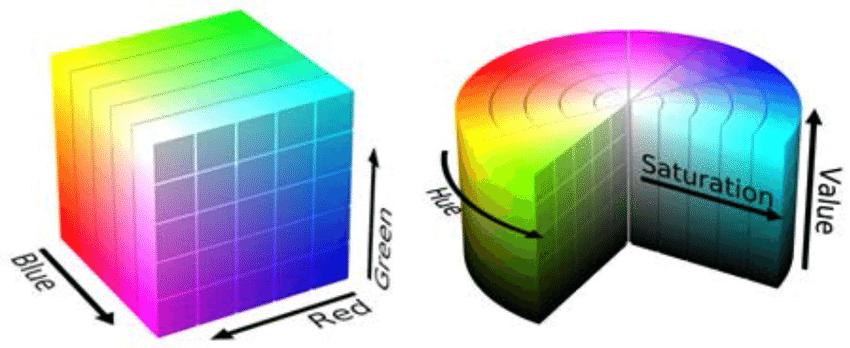
\includegraphics[width=\linewidth]{images/RGB-HSV-color-spaces.png}
    \caption{Comparison of the two most common color spaces (\cite{HVS-RGB})}
    \label{fig:col_space}
\end{figure}

By adding more layers more data can be displayed, such as an alpha channel, which makes the image transparent.
Representing the pixel values has also a couple of methods.
It can also be represented as an integer number or floating-point.
For integer representation usually, 8 bits are used, allowing the values to be between 0 and 255.
This is enough for the human eye to blend the represented image spectrum as a continuous space.
The computer algorithms are however too precise for such low representation therefore a floating-point value is used.
This can be range from 0 to 1 and can take up any value between based on the precision.

The raster representation can be easily displayed, but hard to gather information from it.
For this, the image either should be transferred to the other representation, or pixel-wise information should be extracted by specialised methods.
Converting the image representation can be computationally hard, for example, the Fourier transformation, or the Hough \cite{Duda:1972:UHT:361237.361242} transformation.

The other option is the convolution implementation.
This mathematical formula goes like:

\begin{equation}
    g(x,y) = h(x,y)\star f(x,y) = \sum_{k=-\infty}^{\infty} \sum_{l=-\infty}^{\infty} h(x-k,y-l) f(k,l)
\end{equation}

where g is the output image f is the input image and h is a convolutional kernel.
The transformation is LSI (Linear Space Invariant), commutative, associative, distributive, and associative for scalar multiplications.
In the real-life, both h and f are finite size.
This entails the modifications of the equation,

\begin{equation}
g(x,y)=\sum_{k=1}^{height} \sum_{l=1}^{width} h(k,l) f(x+k-1,y+l-1)
\end{equation}

however, the convolutional filter is usually larger than 1 pixel, thus at the edges, an indexing problem arises.
For this, the image should be extended by $\lfloor size_h/2 \rfloor$.
To do this there is a couple of solution, as filling the missing part with zeros or constants, copying the last pixel of the image or wrapping the image around creating a torus from it (\cref{fig:borders}).

\begin{figure}
    \centering
    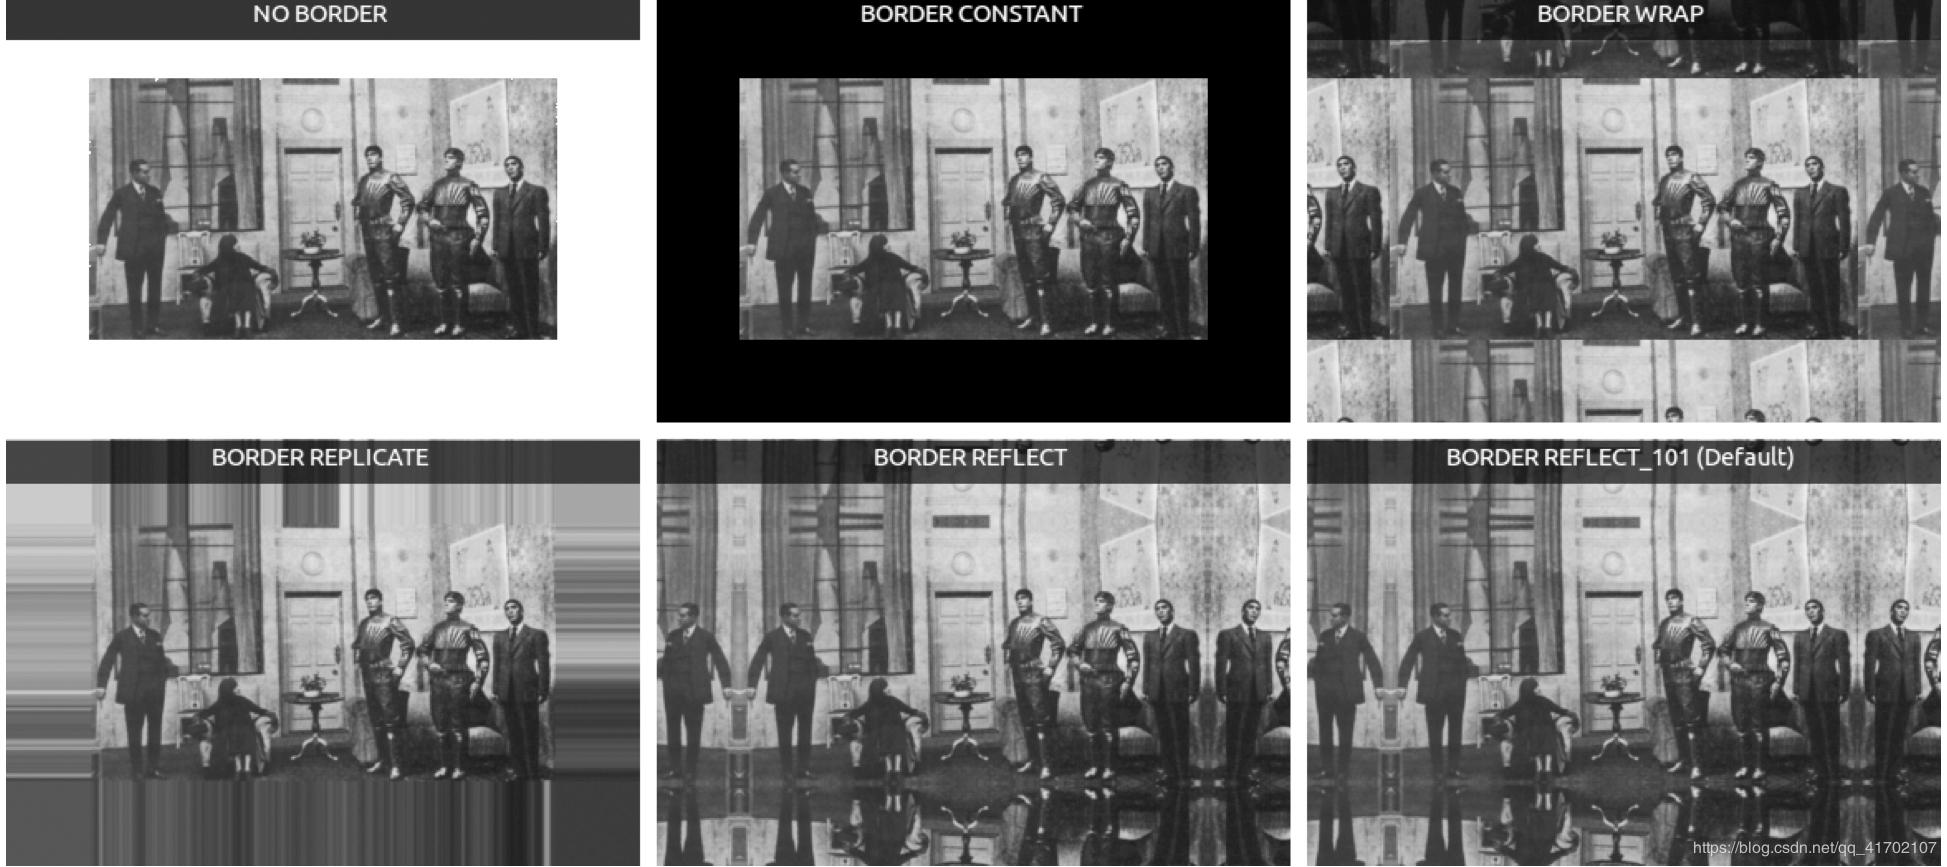
\includegraphics[width=.9\linewidth]{images/borders.jpg}
    \caption{different border types in the OpenCV library \cite{img_border}}
    \label{fig:borders}
\end{figure}

The convolution can be used for different applications, based on the kernel it uses.
As not only the central pixel is considered but the neighbouring values as well, the resulting image transforms in relation to the environment of each pixel.
It can smooth the image, can enhance the edges or blur.

% The greatest advance in the convolution was when as a neural network, the kernel weights was set by a deep learning algorithm.

\subsection{Neural network} % 3742 characters
Deep learning is a buzzword, in the IT industry, for almost a decade.
This is a Machine learning method, for applications where the usual algorithmic approach is not possible.
The basic idea is to copy the learning mechanism of the human brain.
There is a learning set, with some input structure and the corresponding expected result.
The system starts from a random inner state and calculates the outputs.
After a comparison of the expected and actual results, the inner state is updated.
Thus the inner state adjusts step by step to the target function.
For this 3 component is required.
An underlying pattern, which can be approximated by the network, a learning set, to train the network, and a complex mathematical representation that is hard to implement.

Deep learning is a common solution for image classification, since the correlation of the pixels, and the meaning behind the picture is hard to describe through mathematical functions.
For that matter, we also know that the pattern exists, as even a kid can recognise basic shapes and even more complex forms on the image.
The only thing missing is the training dataset and a proper working neural network to learn.
The first approach for image procession was the fully connected network.
In a traditional fully connected network all the inputs are connected to each other.
A pixel of an image has few in common with the other pixels except the closeby neighbours.
This results in lots of computations that have little impact on the final result.
The other problem if the images have some offset.
A fully connected layer considered the exact position of the pixel as an important parameter.
To process the image efficiently a convolutional neural network should be used.

The previously introduced mathematical formula can be easily modified to work as a neural network.
The convolution considers only the kernel size area of a pixel, eliminating noise that was introduced by the presence of the further pixel.
Since all the calculation that should be done is limited to the kernel size, it also uses fewer resources.
The convolution is also capable of changing the dimensions of the image.
Meaning that the 3rd dimension that stores the colour data can be expanded to store other features.
In a convolution operation, there can be more layers of an image, each containing different features.
These features are not always has some physical meaning rather some abstract representation of the image, on which, later decisions depend (\cref{fig:convolvution}).

\begin{figure}
\centering
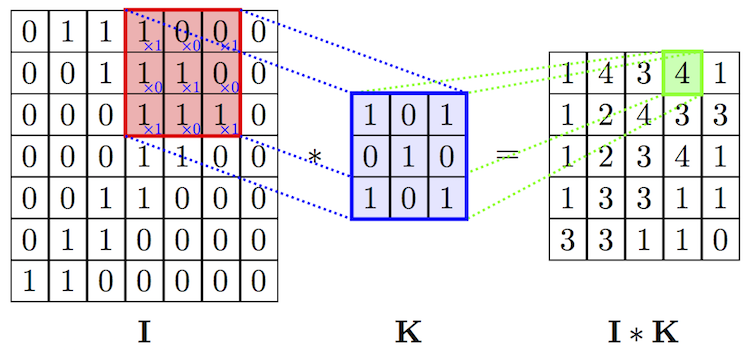
\includegraphics[width=\linewidth]{images/convolve.png}
\caption{Visualisation if the convolution \cite{spark_deep_nodate}}
\label{fig:convolvution}
\end{figure}

The kernel stride determines how small the output image will be.
On every stride step, one pixel is calculated, hence if the stride is 2 then every $2^{nd}$ pixel is calculated.
This makes the output image half of the size of the input image.
This is not a problem for such a system since the required information is not graphical, thus if the smaller image can store the information the fewer resources should be used.

A convolutional layer being an LSI system, can not be chained due to the linear property.
To chain more convolution together the system needs to become nonlinear.
To provide the nonlinearity to the system activation functions are used.
These are nonlinear functions that wired to the summation expression of the layer.
The function can be complex like a sigmoid function or can be a plain rectified linear unit (ReLU).
This ReLU function is a linear function on the positive halfplane, and zero on the negative (\cref{fig:relufunc}).
This property makes it easy to calculate, but still providing the required nonlinear property.

% ReLu
\begin{figure}
\centering
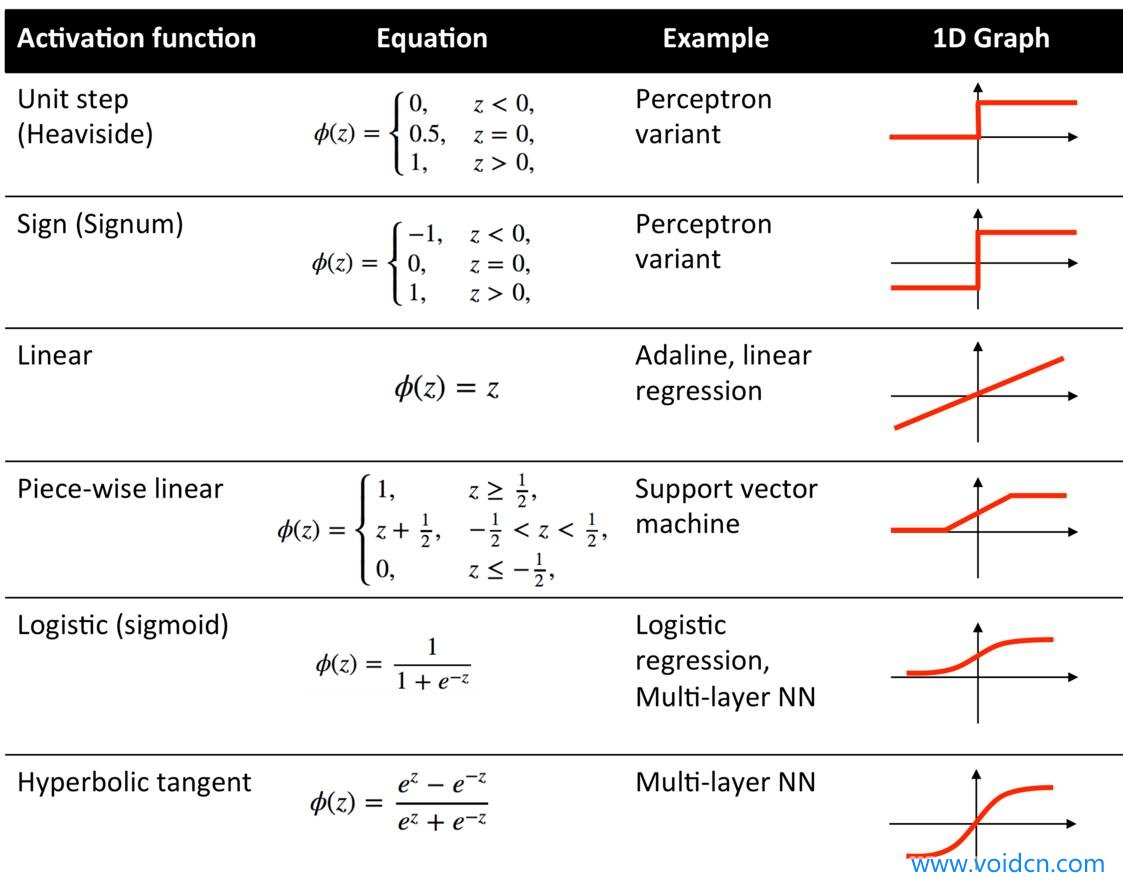
\includegraphics[width=.85\linewidth]{images/activation-functions.jpg}
\caption{examples of possible activation functons in a neural network \cite{sebastian_activation} }
\label{fig:relufunc}
\end{figure}

In a CNN architecture, there is usually another function is implemented.
This function also adds nonlinearity to the system and also raises the most prominent features.
The so-called pooling layer also uses a kernel which strides through the images and replaces the pixel values according to the kernel.
Usually, max-pooling is the most common.
This returns the maximal value inside the kernel.
There are also other types of pool functions like average, or $l^2$ norm pooling.

To do the final decision a fully connected layer is required.
This layer transforms the grid-like values to an array or a single number.
But instead of weighting the pixel values, now it weights features extracted by the previous layers.
Usually, an array is preferred, where the array elements are all the possibilities of a certain output.
The array can be considered the confidence of the network.
This is called One hot encoding

\subsection{FPGA} % 2917 characters
The drones, due to weight limits, unable to carry large power sources, and the computing devices should also be small, light and energy-efficient, hence the GPUs (Graphical Processing Unit) are out of the picture.
Another possible computing platform is the FPGA (Field Programmable Gate Array), more specifically the SoC (System on a Chip).

The FPGA is a circuit consist of a series of logic gates and the programmable interconnects between the gates (\cref{fig:fpga_block}).
The strength of such a circuit lies in its programmability.
With basic logic gates, every function can be implemented.
After designing the function and assembling the logic gates, the final circuit can execute the required calculations and produce the results.
In the traditional development phase, the circuit was implemented in a semiconductor.
In case of an FPGA however, the silicon parts are already in place, only by programming the connections every circuit can be implemented.

The system implemented on an FPGA will of course never be as fast as an ASIC (Application-Specific Integrated Circuit) optimised for the exact task.
On the other hand, the FPGA has not to be reworked from scratch every time a new task is at hand.
Designing new software to program the interconnects, does require less time and less expensive.
An FPGA can also be used for different purposes based on the program.
In comparison to the classical processing algorithms, the FPGA does not use a finite ISA (Instruction Set Architecture), but a low-level gate array.
This gate array can work faster, and can even implement functionalities that are hard or not possible with a traditional SISD (single instruction stream, single data stream) architecture.

\begin{figure}
    \centering
    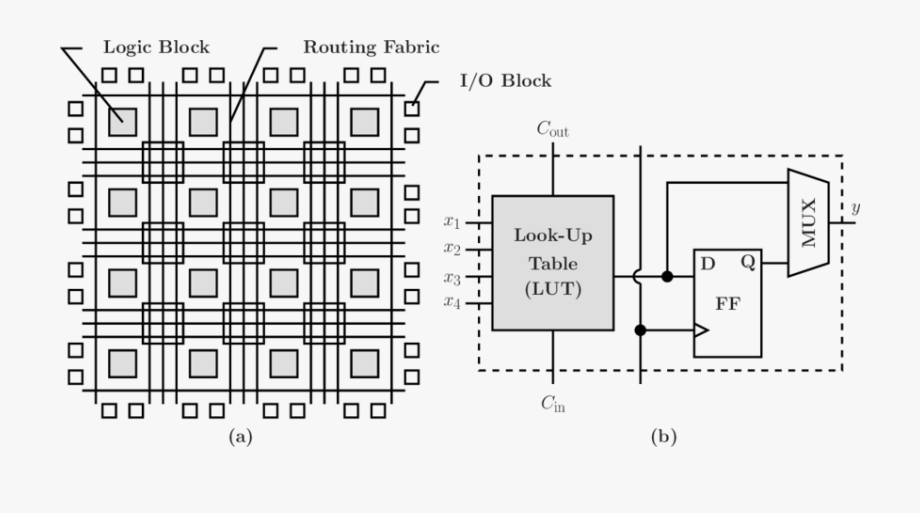
\includegraphics[width=\linewidth]{images/fpga-block-diagram.png}
    \caption{Block diagramm of an FPGA (\cite{fpga_block})}
    \label{fig:fpga_block}
\end{figure}

The modern FPGA chips are usually come with a microcontroller architecture integrated.
This combined system called SoC.
The modern system also changed the basic gate implementations to CLB (Configurable Logic Block).
CLBs can solve more complex logic functions in there own by using LUT (Look Up Table) and contains register as well.
Thus the FPGA reduces the latency closed by the interconnects, and also can function as a memory or temporary storage.
There are also complex arithmetic units included in the CLBs like adders and multiplier units.
By using these bypasses the latency LUT accelerating the system even more.
In the interconnecting part are also implemented a carry propagation connection, which connects the CLBs carry logic parts.
Thus greater adder circuits can be implemented without the carry occupying the connection bandwidth.
DSP (Digital Signal Processor) slices also can be found among the logical blocks.
This block contains simple ALUs (Arithmetic-Logic Unit), accelerating the major algorithms and reducing the CLB requirements of the signal processor applications.
The modern architectures also integrate GPUs and HBM (High Bandwidth Memory) on the same chip.
This ACAP (Adaptive Compute Acceleration Platform) system contains everything for accelerating a modern computational system.
The special task implemented on the FPGA, the calculation tasks are done by the GPU, the cache and buffering loaded to the HBM and the system is controlled by the processor subsystem.
It combines the advantages of all parts without sacrificing efficient programming. 
The configurable SoCs are also small in size and runs on low power.

The thesis discusses a system design that can read the camera images and detect the closing obstacle while running on SoC.

\clearpage % Ez azért kell, hogy nehogy képek átcsússzanak a következő fejezethez
\chapter{Antecedents} \label{ch:ant} % 12486 characters

\section{Avoid system} % 2119 characters
Previously on the University and in collaboration with SZTAKI (Számítástechnikai és Automatizálási Kutatóintézet), there was research for an image-based camera system  \cite{Zarandy2016}  \cite{Bauer2019} \cite{Zsedrovits2016a} \cite{Fuller2014HardwareDA}.

The system consists of three main parts (\cref{fig:Algorithm}).
The first is a preprocessing, which uses well-known image processing algorithms that are implemented in many computer graphic library.
These functions chained together can provide detailed information based on the pixeled data.
For example, the erode function reduces the size of the white areas, by reducing the area by one pixel at the edges.
This helps separate different objects, that may connect.
The opposite of this function is the dilatation.
This adds another layer of pixels at the edge of every white area.
By this, the small objects can connect and act as one.
These two functions applied after each other results the so-called opening and closing effect.
This means that if the erosion separates two objects and the dilation was not able to reconnect them than those two was held on by a thin line of pixels, hence there are two separate objects.
On the Close side, the same stands.
If the merged objects can not be separated by the erosion than those are in reality one object, and the noise made them look like two.
In both Open and the Close cases the objects keep their size, while the noise is removed.
A Gaussian blur convolves the image by a special kernel, which is a discretised 2D Gaussian function.
By applying it to the image, the centre pixel of the kernel has the greatest weight, and the neighbouring pixels are less emphasised.
The thresholding function is a common solution for creating masks.
In this case, the opposite drone should be selected by the mask, and the sky should be hidden.
The image usually contains fine adjusted pixel values, and by thresholding, such an image, the jitter between the values can cause lots of noise on the thresholded image.
Therefore it is good to smooth the image.
This makes the sharp lines blur a little, but that is only visual.
As the algorithm is applied the results became better.

This preprocess phase separates the horizon and the vegetation from the aerospace.
In the separated space bounding boxes are applied to the critical areas (parts of the images that may be dangerous).
From these boxes, a neural network selects the most prominent box.
The selection system is a small network to minimize the processing power required.
The selected box then transferred to a tracker algorithm.
This tracker has a general interface, to change it in later implementation.
For now, it is a simple linear tracker.
The tracker algorithm is returning an assumed trajectory.
The tracker uses the previous positions of the boxes. 
There is also a forgetting factor added to drop old positions.

\begin{figure}
    \centering
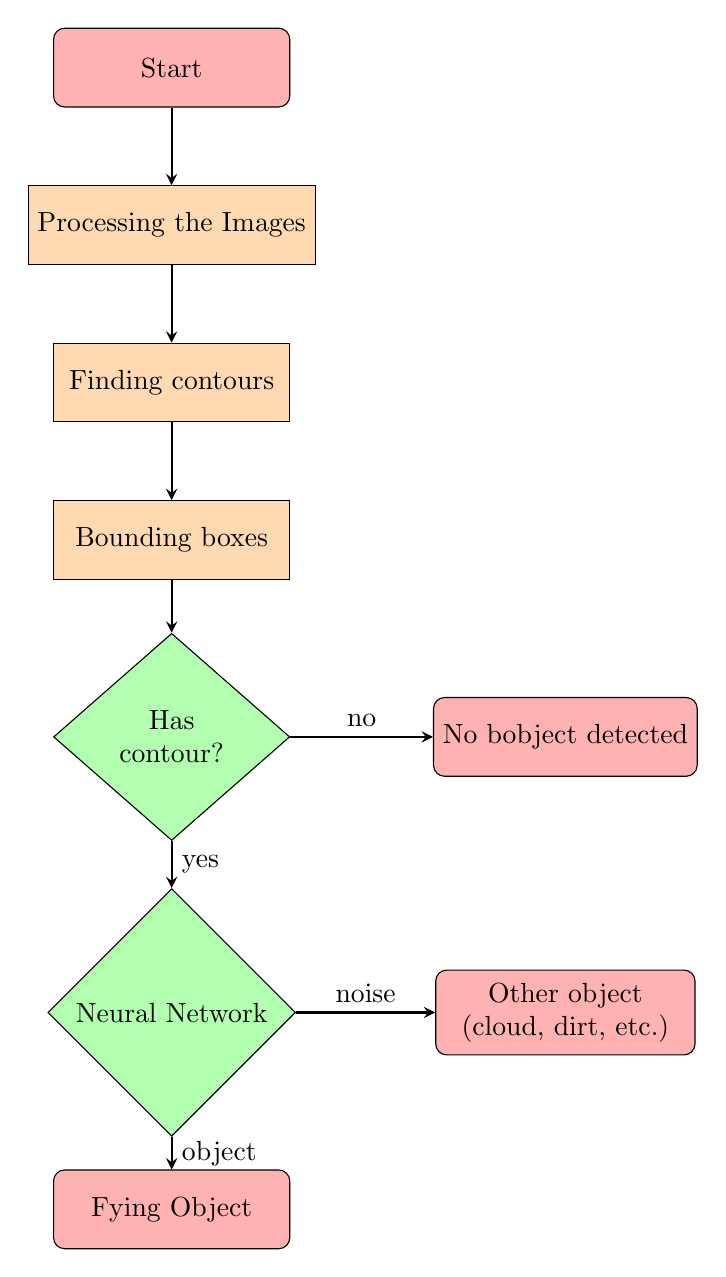
\begin{tikzpicture}[node distance=2cm]
    \node (start) [startstop] {Start};
    \node (improc) [process, below of=start] {Processing the Images};
    \node (contour) [process, below of=improc] {Finding contours};
    \node (boxes) [process, below of=contour] {Bounding boxes};
    \node (decision) [decision, below of=boxes,yshift=-.5cm,text width=1.5cm] {Has contour?};
    \node (CNN) [decision, below of=decision,yshift=-1.5cm] {Neural Network};
    \node (avoid) [startstop, below of=CNN,yshift=-.5cm] {Fying Object};
    \node (ok) [startstop, right of=CNN,xshift=3cm] {\begin{tabular}{c}
    Other object \\ (cloud, dirt, etc.)
    \end{tabular}};
    \node (noop) [startstop, right of=decision,xshift=3cm] {No bobject detected};

    \draw [arrow] (start) -- (improc);
    \draw [arrow] (improc) -- (contour);
    \draw [arrow] (contour) -- (boxes);
    \draw [arrow] (boxes) -- (decision);
    \draw [arrow] (decision) -- node[anchor=west] {yes} (CNN);
    \draw [arrow] (decision) -- node[anchor=south] {no} (noop);
    \draw [arrow] (CNN) -- node[anchor=west] {object} (avoid);
    \draw [arrow] (CNN) -- node[anchor=south] {noise} (ok);
\end{tikzpicture}
\caption{Flow chart of the algorithm}
\label{fig:Algorithm}
\end{figure}

The development of this software reached a satisfying conclusion, as it was tested in a simulator environment, PCs (Personal Computer) and GPUs.
This algorithm was decided to further to a real-life problem.
However, since our flight platform unable to carry a GPU, nor a whole PC, the system needs to be compressed both in size and weight.
At this point, the VLSI (Very-Large-Scale Integration) lab was approached with the request.

The detection system has the requirement of covering 360 degrees of view.
This is necessary to cover every angle of the UAV against any collision.
Usually, the commercially available drones are equipped with only one camera tough a wide-angle one.
That, however, is not enough, hence new hardware should be implemented.
For the first try, the easiest (and commercially available) solution was the GoPro\texttrademark \cite{GoPro} action camera.
It is a wide-angle solution \cite{GoPro_resolutions}, and with 4 GoPro\texttrademark attached through HDMI (High-Definition Multimedia Interface) connectors, the whole 360-degree area can be covered.
The cameras use the same connection interface and are interchangeable, tough is a costly solution.
The more concerning problem is when the 4 separate HDMI connecting to the SoC.
Any system found on the market only provides at most 2 in and 2 output HDMI instead of 4 in and 0 out channels.
This idea is still available however it includes some custom hardware design steps, that are a costly and long process.
At this rate, it was decided on a different approach.

\subsection{LogiBricks} \label{sec:logibricks} % 1230 characters
The first approach to this problem was through the LogiBricks'\texttrademark \cite{Logibricks} hardware system.
The Company creates IPs (Intellectual Property) for Xilinx\texttrademark products and develops computer vision applications for FPGAs.
There is a product, named logiADAK-VDF-ZU\texttrademark \cite{logiVID-ZU} (\cref{fig:logic_4cam}), which integrates 4 cameras with an FMC (FPGA Mezzanine Card) and outputs it through HDMI connection.
On the hardware side, the mainboard is a ZCU102 Evaluation Board \cite{ZCU102} from Xilinx.
For the HDMI connection, the AVNET\texttrademark \cite{AvNet} AES-FMC-HDMI-CAM-G card is used.
The cameras are connected through an FPD-Link-III deserializer board, that connects to 4 OV10635 \cite{Omnivision} CMOS (Complementary Metal-Oxide-Semiconductor) WXGA(1280x800) (Wide Extended Graphics Array) HDR (High Dynamic Range) HD (High Definition) Image Sensor.
The cameras are connected through coaxial cables to the FARKA\texttrademark connectors.
The four channels are connected directly to the FPGA, but the configuration is done through $i^2C$ (Inter-Integrated Circuit) protocol.
For that purpose, there is a MUX (multiplexer) that divides the one serial link to 4 distinct one.
In the first step, the $i^2C$ expects the settings of the MUX, that establishes the channel to the camera.
Then the configuration data can be sent to the selected camera.
This is done by a custom IP which was included with the set.
There were also two other IPs, one for controlling the camera images, the other is for controlling the 4 channel dataflow.
\begin{figure}
    \centering
    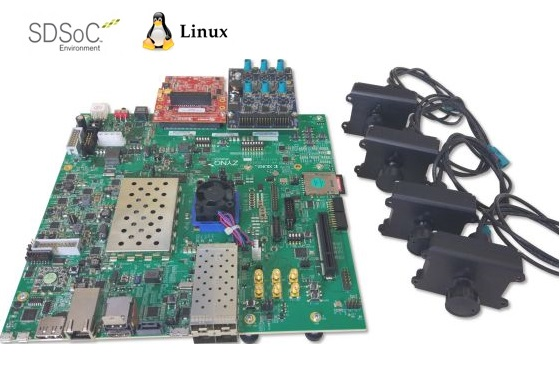
\includegraphics[width=\linewidth]{logiVID-ZU560X.jpg}
    \caption{LogicBricks 4cam system parts \cite{logi_4cam_img}}
    \label{fig:logic_4cam}
\end{figure}

\subsection{Avnet Mipi} % 725 characters
There was another similar device at hand.
The AES-FMC-MULTICAM4-G (\cref{fig:avnet_mipi}), by the previously mentioned Avnet\texttrademark company.
This is also an FMC connected 4 sensor camera system.
All sensor consisted of a MAX96705 16-Bit GMSL (Gigabit Multimedia Serial Link) Serializer and an AR0231AT CMOS digital image sensor with an active pixel array of 1928Hx1208V capable of 4-exposure HDR at 30fps.
This is a smaller sensor than the OV10635 but on the other hand, it can do a better resolution, while not sacrifices the HDR capability.
The lack of cover and the modular assembly, however, makes it more vulnerable.
This system uses an open MIPI CSI-2 serial interface.
Although this system has an example project, the project not used specialized IP blocks.
That way self-made designs are easier with this setting.
This makes the integration of the camera module to the other parts easier.
\begin{figure}
    \centering
    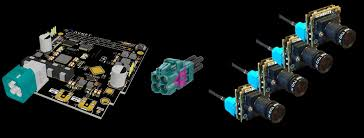
\includegraphics[width=\linewidth]{images/avnet_mipi.jpeg}
    \caption{Avnet 4cam boundle \cite{avnet_mipi_img}}
    \label{fig:avnet_mipi}
\end{figure}

\section{Airsim} % 610 characters
The algorithm that is used for the project is based on a simulator image.
This is the Microsofts\texttrademark Aerial Informatics and Robotics Platform \cite{AirSim} (Airsim for sort), based on the Unreal Engine\texttrademark \cite{UnrealE}.
This is an open-source project that creates a close real environment for testing purposes (\cref{fig:airsim_screen}).
The vehicles can be programmed, to follow a certain path and can be also controlled through an API (Application Programming Interface).
The first is especially comes in hand when the collision is simulated.
It is a hard task to finetune two areal vehicles in the air to collide to each other, in a controlled manner.
In the other hand, the simulator aligns the two trajectories to cross each other, and the record is already usable for the system to detect.
\begin{figure}
    \centering
    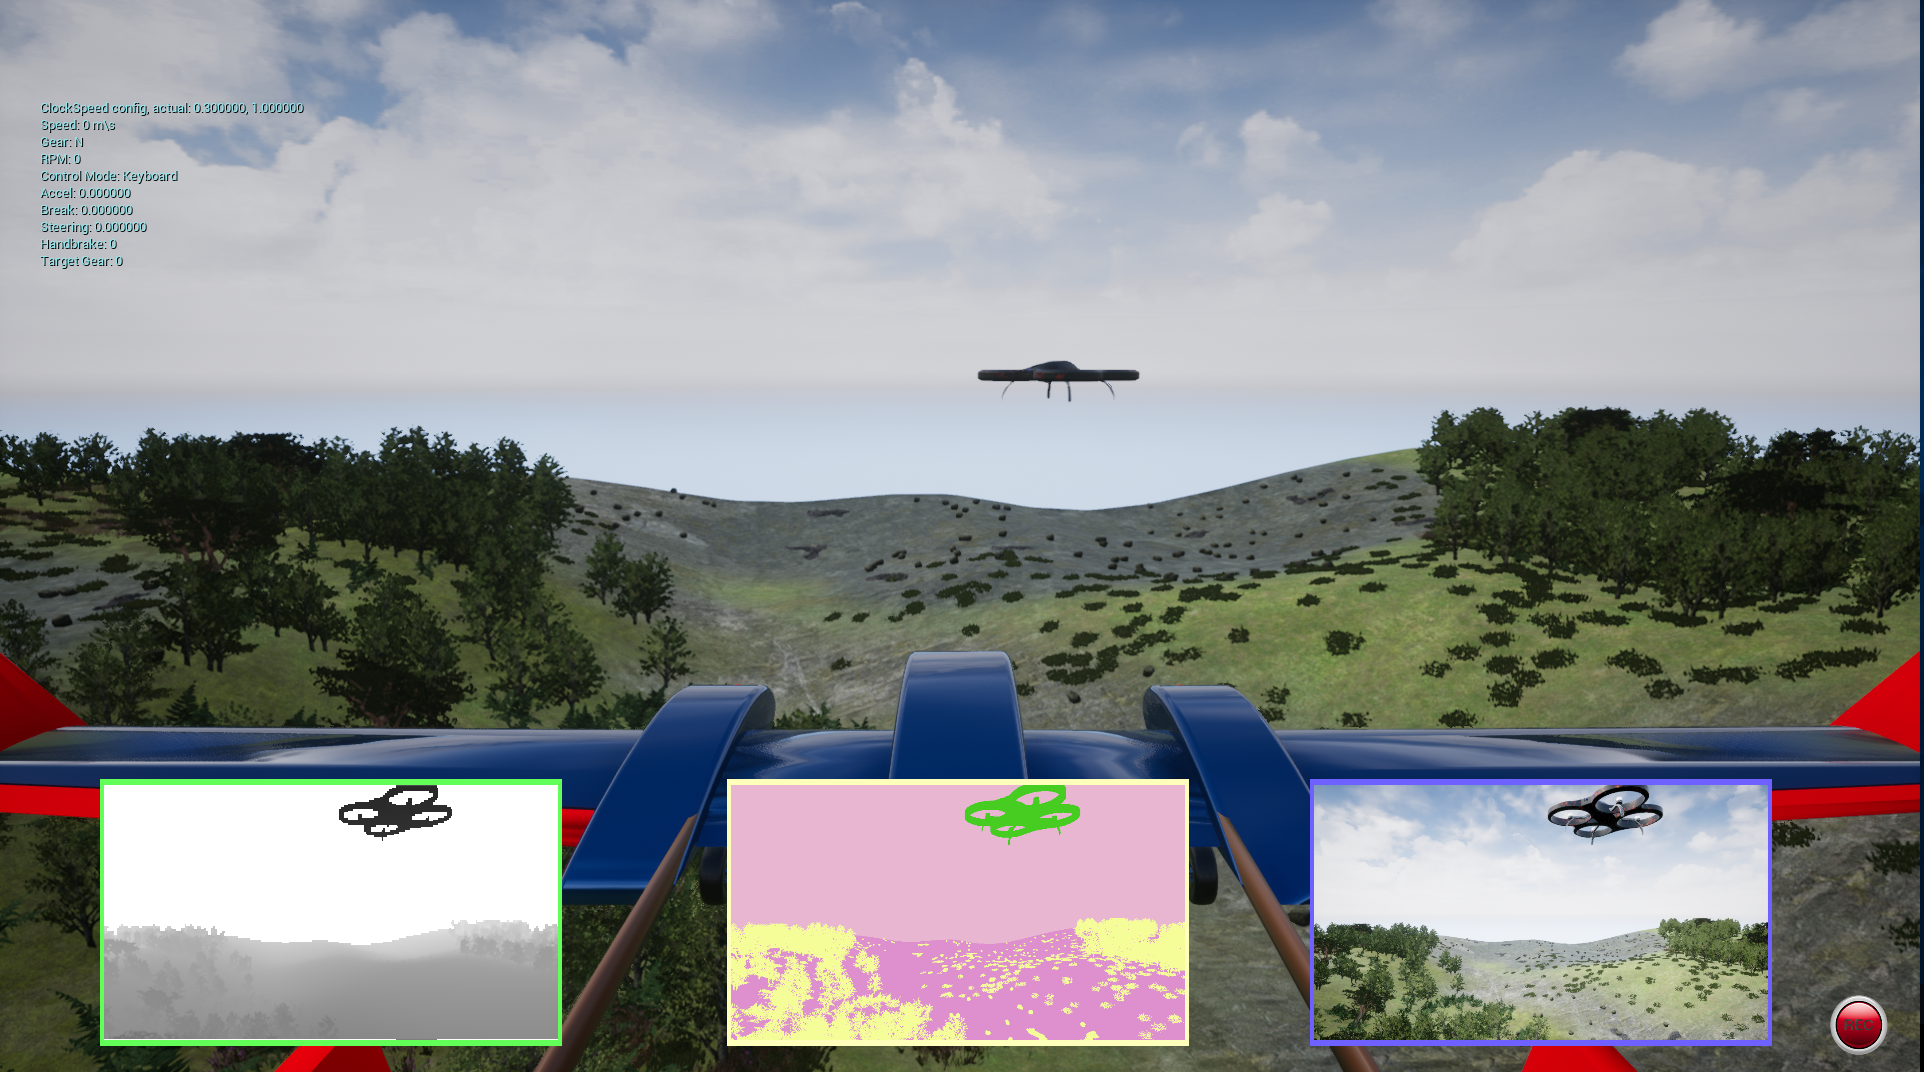
\includegraphics[width=\linewidth]{images/airsim.png}
    \caption{Airsim simulator software screen capture}
    \label{fig:airsim_screen}
\end{figure}

\subsection{HDMI / Ethernet} % 955 characters
There is also a convenient function which is the Ethernet connection.
The API can connect to the simulator through an Ethernet connection using the socket of the program.
This socket can transmit the images from the simulator to the API, which can be processed with the OpenCV (Open source Computer Vision) functions.
This API has a Python and a C++ implementation as well.

The other option to transfer the image to the computing system is through HDMI connection.
The Airsim uses GPU of the simulator server, thus the output video can be redirected to the SoC instead of a display.
For this, there are two possibilities.
The first is the previously mentioned HDMI FMC card from Avnet\texttrademark.
This solution connects the data source to the FPGA directly, witch allows either direct transfer to the output of the same card or accelerated image processing algorithms to applied, limiting the transfer time even further.
There is also an HDMI I/O (Input/Output) port on the ZCU102 as well.
The board has a transceiver subsystem installed, that transfers the data to the PL (Programmable Logic).
For this transceivers, a special programming IP is required.

\subsection{Real flight test} % 409 characters
In a previous conference paper \cite{8798265} the research group described the available hardware.
There are some details of the UAV.
For the real flight test, a 3DR X8+ \cite{x8} (\cref{fig:drone}) will be used, which can carry 800grams.
The UAV is powered by a four-cell Li-Po battery with 14.8V nominal voltage.
There is a DC-DC converter unit onboard, which generates 12V for the FPGA board, and can power up the cameras.
The UAV uses the popular Pixhawk\texttrademark autopilot, which can be connected to the FPGA board through Mavlink protocol \cite{Fuller2014HardwareDA}.
\begin{figure}
    \centering
    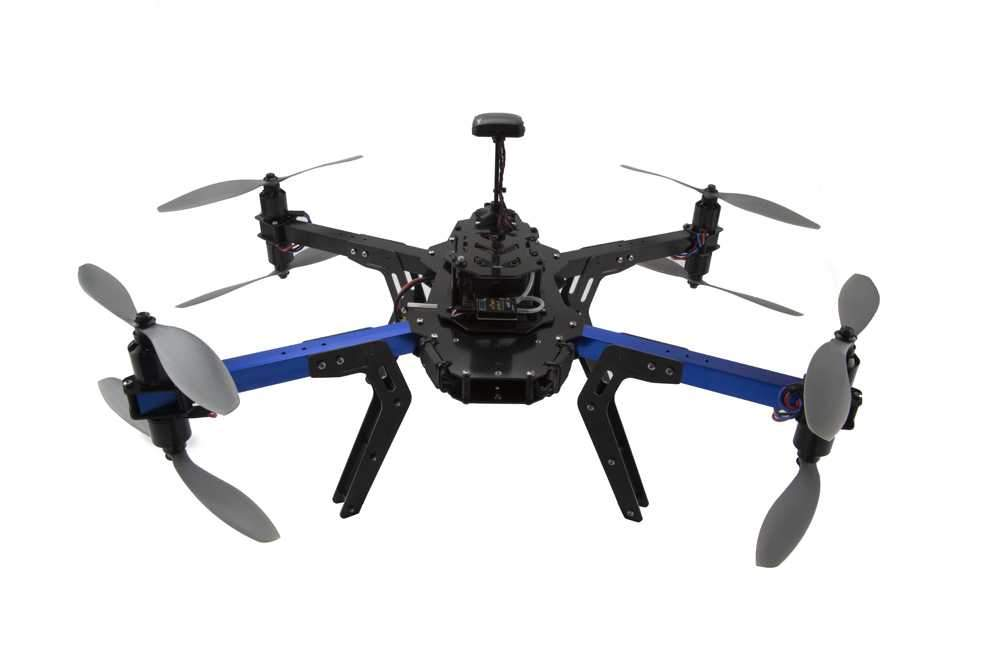
\includegraphics[width=\linewidth]{images/3DR-X8.jpg}
    \caption{The 3DR X8+ drone}
    \label{fig:drone}
\end{figure}

\section{Operating system} % 334 characters
For an embedded system like this, an operating system is required.
Not only the FPGA not working on its own, hence it requires some control unit, but the multiple parts of the whole system require some kind of communication, and execution order.
The PL part could be easily driven by a handmade software, but the loading of the video signals and the other systems requires some higher functionalities.

\subsection{Free Real-Time Operating System} % 955 characters
This operating system is a real-time operating system kernel for embedded devices \cite{FreeROTS}.
The project runs under an MIT (Massachusetts Institute of Technology) free software license.
It is designed to be small and fast.
By limiting the kernel to only 3 files, restricting the allocation policies to strict rules and using multiple threads, the FreeRTOS\texttrademark ensures real-time execution.
This means that by executing a program deterministically, it ensures that the response for an event will be handled in a certain amount of time.
The IoT (Internet of Things) devices and microcontrollers, which are used in automotive systems are required to be deterministic, in order to provide sufficient reaction to the actuators.
In this scenario, the camera input and the control of the drone are both preferred to be deterministic.
Through this OS the drone control can be even transferred to the SoC which saves a computational unit and eliminates one communication connection.

The OS has however little to no support libraries, which makes hard to connect to other systems.
There are also no driver packages which makes hard to connect to the peripheries.

\subsection{Robot Operating System} % 938 characters
The Robot Operating System\texttrademark \cite{ROS} is a Linux Ubuntu\texttrademark based software package, optimised for robotics use.
The OS is modular, and be optimised for low-level device control, hardware abstraction and messaging between subsystems.
It is really good for connecting computer clusters, and embedded devices.
The node like computational graph tough not an RTOS itself provides low latency reactivity.
There are support packages for C++, Python, platform-independent tools and client libraries.
The Airsim environment is also one of the supported packages of the latest ROS.
With this OS the control of the drone could be done as well, even if the original driver unit is not transferred to the SoC, through the communication interface.

The negative side is that the OS is required to run on a full-fledged Ubuntu\texttrademark with all the programs not required by the SoC.
Building the image for a custom hardware architecture, such as the ZCU102 is not as trivial as it seems at first.
The unnecessary parts of the OS, like the simulator environment, also takes up space, and requires resources that are not good for the final product.

\subsection{PetaLinux} % 595 characters
Petalinux\texttrademark is a toolset developed by Xilinx\texttrademark to build embedded Linux systems on the Xilinx\texttrademark processing systems.
In contrast to the previous two, it has drivers, prepared for the Xilinx\texttrademark MPSoCs (MultiProcessor System-on-Chip), and a command-line interface. 
It also includes GCC compiler tools for debugging and system image-building purposes.
The image builder is designed to prepare the BSP (Board Support Package) with only the necessary drivers and libraries.
Through the tools, the Linux kernel can also be altered to the proper purposes.
Asymmetric Multi-Processing (AMP), the possibility to run different tasks on each processing core, is also available, as well as a real-time approach and Xenomai\texttrademark \cite{Xenomai}.

\subsection{PYNQ - Python productivity for Zynq} % 1427 characters
Thy PYNQ \cite{pynq} system is a Python-based development environment for Zynq-7000 SoCs and MPSoCs.
This open-source project is making embedded design easier for high-level programming.
On the processor, a basic PetaLinux\texttrademark and a Jupyter\texttrademark \cite{jupyter} notebook server are running.
This allows the developer to write the algorithm in Python, and run it on the processor, and later accelerate it with the PL part.
The acceleration is done by so-called Overlays.
These overlays are IPs blocks that designed to accelerate time-critical functions of the system and runs on the FPGA part.
Such an overlay is usually developed using VHDL but the software that controls the device can be implemented in Python instead of a standalone C++ application.
The PYNQ system also provides prebuilt overlays, that has an already implemented interface, hence on the Python side, only the function call is required.
On the platform, there is a lot of community-driven projects, of different overlays, such as xfOpenCV which implements OpenCV \cite{xfOpenCV_pynq} functions on PL, or the BNN \cite{finn} which is a framework for a neural network using only binary weights and still performing in a small margin of error, and lot more \cite{rybalkin2017hardware}.

The negative side of the system that is not supported on every board.
On the supported platforms, the usage is easy, but on not supported systems the OS and the overlays must be build from source.
The already built IPs has drivers, the PYNQ system recognises these, and allows access to them through simple function calls.
There is the possibility to design other IPs, but those are not always work properly, and had to program them manually.
This requires the user to write the python wrapper functions, that are already done for the prebuilt overlays.

\section{FPGA development}

\subsection{High-level synthesis} % 503 characters
The HLS (High-level synthesis) is an automated design process to generate hardware systems.
The user has to describe the algorithmic description of the required system in a high-level programming language.
This serially executed code is converted to the parallel executable hardware description, through directives.
The software than transferred to an RTL (Register-Transfer Level) description.
This includes the routing and the required Electric parts, as well as the timing and clocking.
For Xilinx\texttrademark products, the Vivado HLS\texttrademark also creates drivers for the generated IP block for easier integration.

\subsection{Vivado} % 1072 characters
The two main manufacturers of FPGA is Intel\texttrademark (formerly Altera) and Xilinx\texttrademark.
The University chose to contract with Xilinx\texttrademark that has a slightly more market share.
The Xilinx\texttrademark FPGAs are shipped with the corresponding software and developer tools.
To program these devices, either a hardware description language or prebuilt building blocks must be used.
The Vivado Design Suite\texttrademark is a complex developer software, that allows the users to use either VHDL (VHSIC-HDL) (Very High Speed Integrated Circuit Hardware Description Language) or Verilog languages, to design their software.
Verilog is closer to the hardware level, VHDL allows more abstractions.
Both are useful to create functionalities.
These code blocks can be imported to block design.
This graphical programming interface allows the users to wire the already working blocks together for more complexity.
In the block design, there also can be included the prebuilt and optimised IP blocks of common applications, like memory access, interconnections, clock generators or the processor subsystem for the SoC devices.
There can be developed also testing circuits, which generates signals and can simulate the working circuit.
This step helps the developer to avoid bugs or even dangerous commands in the hardware design.
The simulation also speeds up the development, since there is no need to program the device every time, can be done offline and allows detailed examination for the signal changes.
The synthesis can be run if everything works properly.
The synthesis compiles the hardware description and creates a theoretical circuit.
This circuit thus uses the building block included in the FPGA but generates a generally implementable system.
To became device-specific, the synthesised circuit must be implemented on the selected part.
This circuit describes the exact wires and gates the program will use.
The implementation cannot be transferred between devices as the synthesis.
Finally, the implemented circuit should be written to a bitstream file.
This bitstream is the configuration file for the programmable interconnect and the CLBs.
This is a binary file that can be loaded to the device.
The programmed device can be also monitored through USB (Universal Serial Bus) connection with the Vivado\texttrademark.
If the design includes chip scope debug signals, these signal also can be followed by the Vivado\texttrademark debugger waveform display.
Some bitstream requires the processor subsystem to provide a software extension.
For this, the SDK (Software Development Kit) is used where the C++ code can be written and program the hardware as well as the processor.
Amongst the SDK setting can be also set the base OS, program is designed, and the software source will be copiled to that. 
This can be one of the previously mentioned PetaLinux\texttrademark solution, a custom operating system or a standalone application.

\subsection{Software Defined System-on-Chip} % 614 characters
The SDSoC\texttrademark (Software Defined System-on-Chip) is a Xilinx\texttrademark developer program that combines the HLS and the HDL steps.
The algorithm is written in a high level (C++) language and the program creates the IP blocks according to the directives given in the code automatically.
There also preprocessor branchings that separated the hardware implementation from the software.
This marks for the automated workflow, which part should be simulated in the Vivado\texttrademark project, and which will be the basis of the driver.
The resulting system can be transferred to an SD card and be run on the SoC.
This workflow is easier for a fast and small project but it takes the freedom of creating the hardware part.
It also makes it harder to integrate such a system.

\clearpage
\chapter{Planning} \label{ch:plan} % 21758 characters

\section{Concept and Ideas} % 260 characters
The first step of developing a device is to decide on the specifications and functionalities.
For this, the First step was to approach Dr. Antal Hiba, one of the developers of the used algorithm.
Since he was a previous doctorate on the University, he was eager to help and provided his own Python implementation.

\subsection{The Algorithm} % 2274 characters
Previously the research group of the embedded system laboratory of the university developed an algorithm to track the trajectory of a flying object.
This system is also used to determine whether the trajectory is crossing the path of the drone or it avoids it.
The Python code is tested on the Airsim simulation.
The simulation can be adjusted at the beginning to cross the other drone on different angled trajectories and can be started via a button push.
Connecting to the simulator server via Ethernet connection, the client machine can run the code, that prints on the client-side display the image of the simulator, the detected bounding box and the resulting trajectory.

After connecting to the server, the client requires an image from the simulator.
The simulator can provide multiple data, including 5 camera angles (front-left, -centre -right; bottom; back) and in some models, there is a driver view as well.
With the computer vision settings, it also has Depth Vision, Depth Perspective, Segmentation, Surface Normalized images.
However, for our purposes, the Scene view is only required, which is the visual front camera of the drone.
This image is considered the equivalent of the camera image of a real-life drone.

The images are converted to the OpenCV \cite{opencv_library} data format.
After removing the alpha channel, a preprocessing algorithm is applied.
For easier calculations, the image is converted to grayscale.
This algorithm is consists of many well-known image processing algorithms, such as gaussian blur or erode.
The preprocessing step separates the horizon and the aerial spaces, reducing the area where the algorithm should calculate.
The aerial space then searched for possible dangerous objects, by reducing the images to edges and contours \cite{31447} \cite{SUZUKI198532}.
For the dangerous parts, bounding boxes in OpenCV are determined, and these boxes are returned to the main block.
Usually, these boxes are containing cloud fragments, birds, aeroplane contrails, etc.
The most prominent box is selected by a small CNN (Convolutional Neural Network).
All the boxes are run through 2 layers of 2D convolutions and 2 fully connected layers.
Both convolutional layers are using $3\times 3$ kernels, the first with 10 output layer, the second with 5.
The fully connected layers have 128 and 2 output channels respectively.
The 2 output at the end of the CNN is one-hot-encoded confidence of whether the object is dangerous or not.
By selecting the highest confidence, the most dangerous object is selected.
By applying the same algorithm to the adjacent frames, the change of the bounding boxes can provide a trajectory.
To determine the trajectory a simple linear tracker is applied.
This tracker stores the previous data and tries to predict a track.

\section{Camera system} % 401 characters
For the project, the main goal is to run this algorithm on a live system.
The input image, in this case, will be a camera image.
The easier solution is to use the camera of the drone, however, it has a limited view only.
The GoPro approach is a possible solution of this problem by providing a device available off the shelf, and an interchangeable sensor.
This, however, is not a viable solution due to the requirement of a lot of HDMI connectors.
There should be an imager system in place.

\subsection{LogiBricks} % 2306 characters
In \cref{sec:logibricks} are described as the primary target of the project.
The SoC is fairly large, and has resources for supporting huge applications, like processing several HD images.
The camera system can record $360^{\circ}$ images, and the attached cards are securely connected and bolted to the baseboard, reducing the chance of accidental disconnects.
The FARKA connectors are also automotive ready and securely attached.

At 19th November 2018, the system arrived and assembled in the laboratory.
There was a prebuilt SD (Secure Digital) card image included which can be plugged in and run without any difficulties.
The cameras and the connectors were working properly.
However, the example project had a couple of issues.
The versions of the shipped IP-s were not met, which was corrected by the company by sending a new download link.
After the licensing and the version problems solved the block runs were throwing errors at the implementation phase.
In the video-control block the use of the {oddr\_inst.u\_pix\_clk} resulted in a "cell are unresolved black boxes" error.
Since the IP core was classified no change in the internal system was allowed.

The video controller IP is responsible for saving the video streams to memory and reading it from it.
This method can be easily replicated with basic IP cores, so a hand made solution was created.
The block design expects an image stream from the FMC module, and pixel by pixel saves it to the memory via a VDMA (Video Direct Memory Access) block.
The VDMA converts the streaming pixel data to a memory-mapped image format.
It also processes control signals such as horizontal and vertical sync, active video or blanking for re-synchronization after losing input video data.
From this streaming video data flow, the VDMA creates memory-mapped data and stores it in the onboard DDR memory.
This can also work in the other direction where the VDMA reads the memory-mapped data and converts it to a stream with the corresponding control signals.

The other issue with the handmade solution is the IIC configuration.
The cameras are in a sleep mode state by default.
To get the image data, the cameras should be wakened and set up properly.
This is done through an IIC mux that directs the control signals to the correct camera.
This IIC block is also a LogicBrick\texttrademark IP shipped without documentation.
Since no programming guide was found to the camera control board, the code was reverse-engineered from the added example project.
The resulting code was maybe good but since no bitstream was generated it cannot be tested.
The reverse engineering cannot be tested as well, due to the complex software.

For the future, a working block design must be created and the IIC control code should be tested.

\subsection{AvNet MiPi} % 1539 characters
After the failed attempt on the Logibricks\texttrademark camera system, another similar system was introduced. 
The Avnet\texttrademark \cite{avnet_HUG} company uses the same approach.
The kit also securely bolted to the baseboard, and FARKA connectors are used as well.
This system, however, uses an open software approach and provides sample projects as well as programming guides.
The board transfers MIPI standard video data through the FMC connector.

To use this system the a MIPI D-PHY block is required to process the clock-forwarded synchronous MIPI CSI-2 link protocol.
This provides high noise immunity and high jitter tolerance.
It is also implemented by Xilinx.
The IP has an example design where the incoming MIPI camera signal is transmitted to the HDMI connector.
This example design, however, has some IPs blocks that are bounded by licence thus a D-PHY system was assembled by hand without the HDMI part.

Assembling this system reveals another problem.
The MIPI card pin settings that are described in the programming guide does not correspond with the Xilinx recommendation.
In order to connect to the card, the pin setting should either be set according to the Xilinx settings, that results in an invalid input source error in the program.
It is also dangerous for both the card and the ZCU102 as well, since the connections can be overloaded due to the programs.
The other option is to set the pins as the programming guide, which case the Vivado\texttrademark does not allow the bitstream generation process due to critical warnings.
There was also example projects found on the internet, that resulted in the same errors.
Xilinx\texttrademark also provides an example project for another MIPI card but both the manufacturer and the assembly is different.
The two cards are definitely not interchangeable, thus he configurations are not compatible with each other.

\subsection{HDMI I/O} % 1530 characters
There was also an approach to transfer the image data from the simulator to the image processor via HDMI.
This was first implemented with the Avnet AES-FMC-HDMI-CAM-G card \cite{avnet_HDMI}.
The HDMI converter chip on the card uses the ITU-R Recommendation BT.601 or 709 colour space, and for transmitting this it uses the ITU-R BT.656 digital video protocol.
This standard includes the horizontal and vertical signals into the data stream.
This allows transferring of uncompressed data, both parallel and serial.
Originally the system is designed for digital TV.
In this case, the serial is used which requires 13MHz per pixel transfer speed.
The card also uses the serial approach.
The pixels are encoded to 16 bits based on the YCrCb 4:2:2 standards.
At each clock comes either a YCr or a YCb value pair.
Both the Y and the Cr and Cb are encoded in 8 bits hence the 16-bit bandwidth.
This reduces the 24-bit requirement of the VGA (Video Graphics Array) connector.

For such transmission, the Xilinx provided IPs are still in preproduction, but it can be used.
However, the example project has some IP that the University license does not cover, so no block is generated.
To overcome this obstacle a hand made solution was introduced again.
The previously introduced VDMA connects to a Video AXI (Advanced eXtensible Interface) controller and stores the video to the memory.
On the other side of the AXI controller, a VHDL module feeds the streaming data.
This module is responsible for generating the control signals for the video data.
The control signals are calculated with a shift register that shifts the video data by 4 clock cycles.
These cycles are enough for the detector subsystem to recognise the EAV (End Active Video) and SAV (Strat Active Video) signals.
After such signal is detected the correct control signals are transmitted according to the inner state of the block.

\section{Python environment} % 242 characters
For a final solution, the Ethernet solution was implemented.
The PYNQ system tough works well for the dedicated boards, the ZCU102 is not one of them.
For this, the Operating system should be built for the custom hardware.
The foundation of the OS is a Petalinux, and it runs on Jupyther notebook.

\subsection{ZCU102} % 2581 characters
To build a system for a custom architecture requires a lot of superuser actions.
For safety it is recommended to use a virtual machine, not to ruin the working OS in case of any error.
The supported boards are easily built through a setup script that set all in place in a couple of hours.
For the not supported board, the setting must be done by hand.
First of all, some packages need to be installed or updated, based on the Ubuntu version the VM (Virtual Machine) is installed.
Most of the systems are general, like the python, Jupyter and the Linux OS.
These parts are built separately from the device-specific parts.
The OS can be compiled for arm and aarch64 systems.
This is decided by the config files.
There also can be added other OSs, by creating new folders and including the required bootstrap files.
In the Makefile, the PACKAGE\_BUILD\_\$\{PACKAGE\_NAME\}\_\$\{ARCH\} specifies the package to install and for what architecture it is compiled.
For different OS and special boards, the parameters should be set before the making process.

For the board-specific parts, the PYNQ has a boards folder.
All the supported boards have here a subfolder, and for the custom boards also need to be created one.
In this folder a .spec file sets up 3 crucial variable \texttt{BSP\_\$\{BOARD\}}, \texttt{BITSTREAM\_\$\{BOARD\}}, \texttt{STAGE4\_PACKAGES\_\$\{BOARD\}}. 
These variables are set up the board-specific settings, like the BSP (Board Support Packages) which is a description of the custom device, including the drivers and libraries.
All the software are connecting to the BSP, and the BSP connects to the hardware.
The bitstream contains the programming information for the FPGA.
The stage 4 packages are the packages that are required to compile board-specific, but it is the part of the OS, like ethernet, USB or display devices.

The two kinds of Xilinx SoCs is Zynq-7000 and Zynq UltraScale+.
For these, the arm and the aarch64 architectures are used respectively.
Both systems work properly with the PetaLinux prebuilt BSP, thus no image should be created.
However, if specified BSP is required then a Viviado project should be created and from than a .hdf file is generated.
If the .hdf file is copied into the petalinux\_bsp subfolder, it will be automatically included to the final BSP by the compiler process.
The custom packages are placed in the packages folder and transferred to the compiled system.
This is a convenient way of installing custom notebooks or Python packages.
make BOARDDIR=<absolute\_path>/myboards starts the building process of the custom system in the parameter myboards folder.

The created image copied to an SD card, and after a couple of settings on the board the system boots.
By default the board has a fixed IPv4 (Internet Protocol version 4) address, thus it can be accessed through a client PC.
The Jupyter server runs on the 9000 port and can be accessed with the user password combination defined in the config file.
After accessing the notebooks, the Python environment is ready to use.
The Jupyter environment also provides a root terminal to the system which makes it easy to control the OS.

\subsection{PYNQ overlays} % 2532 chatacters
For the working PYNQ system, the python codes were implemented easily.
Since the PNYQ image came with OpenCV preinstalled, the Airsim and the Chainer was the only missing packages.
Since the system runs from an SD card, the minimization of the package requirements were essential, sine lot of installing and writing to the card may harm the hardware.
This thesis is oriented in the image processing direction, that why the neural network and the tracker subsystem is not required to be installed.
With eliminating the two main part of the system, the Chainer package becomes obsolete.
The Airsim package can be avoidable as well if the images are uploaded to the SD card, for testing purposes.
This, however, does not provide different images in every iteration.
For easier integration and to properly validate the system the Airsim package was installed.

The PYNQ system core is running on the processor architecture and supports the Python code form there.
Since the whole code was written in Python, the algorithm is running on two-arm cores.
With this the computational power is extremely small, resulting in a 2 fps (frames per seconds) processing speed.
The speedup, however, lies in the FPGA part that in this case, it is not even in use.
To use the FPGA part of the chip the PYNQ system provides an Overlay library.
This is a .bit file compiled for the FPGA and loaded to the Jupyther notebook.
Along with the bit file, there should be a .hwh file as well.
The HWH (HardWare Handout) describes the block design as an XML (eXtensible Markup Language), which helps the PYNQ system to provide functions, called register map, for controlling the IP.
This is similar to the traditional workflow where the Vivado creates a header file for the C++ software implementations.
With this register map, the endpoints of the blocks can be driven.

Such Overlays can be found on the community-driven forum page of PYNQ.
People around the world are creating open implementations for numerous tasks, including physical simulations, data mining applications, neural network implementations and image processing algorithms.
These community-driven overlays are usually compiled to the supported PYNQ boards, which not includes the ZCU102.
To use it the codes should be compiled for every overlay.
This may result in a bit of bothersome extra work but nothing more.
However, the image processing project is just a port from an HLS implementation to the PYNQ.
For that, the so-called xfOpenCV which is the Xilinx implementation of the C++ OpenCV, can be implemented function by function to the FPGA.
This saves a lot of work and can speed up even further.
Since the xfOpenCV contains all the functions, it is a huge library, with lots of unnecessary functions for our project.
As for the overlays, there can be implemented a specific preprocessing overlay.
The final preprocessing overlay will require the image and puts out the final processed product.
In contrast to the function by function solution, the Overlay connects the functions inside by a dataflow.

\section{Image processing} % 887 characters
For the image processing tasks, the OpenCV Python implementation is used in the original system.
This is a common and well-used solution.
Since it is open-source, everyone can compile the source for any machine.
In this case, the software implementation of the OpenCV is running on the ARM processors of the ZYNQ Ultrascale+ chip.
The fixed hardware executes the code as any normal processor architecture, so in this case, it is called a software implementation.
The function is implemented on the FPGA, the output is not generated by one or more similar processing cores but loaded to application-specific hardware.
In this case, the wires and the LUTs (Look Up Tables) are directly responsible for the output product.
Therefore this system cannot be used to anything else but the same function every time.
This function, however, is not limited by the Fetch Decode Execute instruction cycle, nor the data-to-memory-copy latency.
This gives the advantage over the SI (Single Instruction) processors, resulting in less power use, and higher processing speed.

\subsection{xfOpenCV} % 2823 characters
The OpenCV implemented to the SoCs by Xilinx is the xfOpenCV.
This contains over 60 functions similar to the original OpenCV implementation but optimized for programmable logic.
The library is also open-source, and free.
The main part is written in C++ and can be used with SDSoC.
In the SDSoC workflow, the C code is compiled for FPGA, a Vivado project is automatically generated, and the driver software is exported in one go.
This makes the work of the top-level designer easier but hides all the intermediate steps.
This is not good for us since the output product here is a full-fledged design running on the FPGA.
For a PYNQ system, the end product of a Vivado project is required, and the corresponding driver software is written in Python.

In the xfOpenCV, there are example projects for every function implemented.
These projects are designed for SDSoC but can be imported to an HLS project.
The function needs to be reworked since the type of the input and output images are xf::Mat template class.
Such a template class is transcribed as an AXI Master interface, and since all fields of the class are transferred the resulting connection becomes unnecessarily complex.
To solve this issue there are helper functions, that transfers a cf::Mat to a hls::stream format.
This stream transfers the image pixel by pixel to the processing function where another function assembles the image again to an xf::Mat.

After this tricky roundabout, the image processing step is ready to start.
The system is designed as a dataflow, which means that the adjacent functions save there results in a temporary variable and the next function uses this result as an input.
For this, the FPGA \#dataflow directive provides an implementation, which uses no memory between the functions.
The function instead of writing the output to an allocated area (as in the SI case), created the interconnect configuration of these functions to be wired together.
This results in a system that is compact from start to end and uses as less resource as possible.

The negative side is that every data object can be invoked 2 times in the code, first when it is written into, and second is when it is read from.
In the original algorithm it is not a problem since every function has an input and an output, however, there is a lot of function that may hard to work with.
Such a method is the Otsu \cite{4310076} threshold calculator function.
This function requires an image and some calculations later determine an optimal value for thresholding.
After the value is determined a threshold function can be called to the same image with the Otsu parameter.
With this method the input image is read two times and is written only once, hence it breaks the dataflow requirement.

This example of the Otsu method is came up as the solution to another problem.
The problem that there is no Adaptive Threshold implemented in the xfOpenCV.
In the original algorithm after a Gaussian Blur, there is an Adaptive Threshold \cite{pratt2001digital} \cite{yanowitz1989new} applied.
This is a convolutional algorithm that uses a kernel to determine a local threshold value.
This local value is more relevant at the small area of the pixel, hence it can result in a more pronounced result.
It produces better results on images with poor lighting conditions, or at low pixel values differences.
The algorithm chose to use this algorithm, in order to eliminate the one-sided illumination of the sun.

\subsection{Threshold} % 2068 characters
Since it was not implemented in the xfOpenCV package, the first approach was to create one.
For this, the already implemented convolution function was used.
This convolution uses a custom kernel and the result is printed to the output image.
The kernel in the case of the adaptive Threshold should be all ones, so in the final implementation, it can be optimised out.
For that, the kernel was fully removed.
The other difference is the thresholding part.
The convolution only calculates the mean of the pixels, the threshold also compares the calculated mean value to the original pixel.
This step must be done inside the function to satisfy the dataflow requirements.
For this, at the end of the convolution, a new condition should be applied to the output value.
It either returns zero or the max value of the image representation (in this case 8-bit unsigned integer).
In the OpenCV implementation, there is also a delta value that allows a small differentiation from the mean value.
However, after adding the required modifications to the solution, the result was not satisfactory.
It either can be, because of the number representation on the FPGA, or the complicated method in the original OpenCV implementation, that calculates the output value.

The other approach was to replicate the OpenCV original function on the hardware.
The already implemented box filter works flawlessly in the example design resulting in a 1.616923 \% error rate.
This is the result of different border conditions.
xfOpenCV only implemented the constant border values, in the original, there is a replicate border.
It also can be seen on the differential image.
The code continues with a double cycle comparing the two images.
The decision between the output value is weighted by a delta parameter.
After the decision, the final images differ about 1-9\% error.
The problem partially comes from the border condition, however, does not explains everything.
With these mixed results, the adaptive method had to be abandoned.

The final result was done by a simple threshold function, with an arbitrary 128 threshold value.
This provides an image clear enough for the algorithm to still detect the drone.
It is a necessity to alter the original system, but since it works as well, it can be used.
The threshold function requires less resource since it does not involve any convolution.
For that, the resulting system will require less resource, and it has to be considered at the calculations.

\subsection{Convolution} % 728 characters
The convolution on a 2D image is done by a 2D kernel as well.
For this, the image is loaded to the mixer function pixel by pixel, and by every pixel, the neighbouring pixels as well.
In case of a $32\times32$ image, and a $3\times3$ kernel that requires $9\times32\times32 = 9216$ pixel loads.
In reality, however, it can be calculated which pixel will load next.
By reserving two memory buffers to store two lines if the image, the pixels can be loaded to them, and propagated in every calculation step.
This results in higher memory use but limits the pixel loading to $32\times32 = 1024$ for the image.

Though the resource requirement of loading the picture is minimized, the calculation still requires 9 multiplier circuit, in a case of a $3\times3$ kernel, as well as an adder.
With this, the difference between the regular and the adaptive threshold are easily be measured.

\section{Decision making} % 788 characters
The algorithm also contains a decision making neural network, which also can be accelerated by the FPGA part.
The task is to create a system that runs the CNN on the FPGA.
For the classification task, only the forward part of the neural network is required, the idea is viable.
On the other hand, the network has to be taught, and weights should be generated for the kernels.
This part raises some problems already.
Since the FPGA uses a streaming data structure, it is hard to save the inner states of the hidden layers.
As the CNN is synthesised to the device, the inner layers either became wires, that can not be read during the run or should connect to memories.
These memory cells can be read with a backpropagation algorithm, but it slows the system.
By introducing memories in the system, at every step a read and a write operation should be done, thus the main purpose of the PL is lost.
Hence the training of the network should be done offline, on a PC.

\subsection{BNN} % 799 characters
Among the Python community systems, several libraries implement neural networks.
One of them is a really interesting approach.
According to the paper, the neural network contains redundancy, and this handled using binary values instead of floating-point.
In the first place, this saves a lot of memory, hence instead of 32 bits there only 1 or 2 is stored \cite{NIPS2016_6573}.
More important is, however, that for the FPGA the floating-point implementation is hard, and requires a lot of resources.
The 1-bit implementation, on the other hand, can be implemented by simple logic functions.
On a GPU and a regular processor, this does not mean a huge advantage, since the instructions in these cases are fix sized \cite{7929192}.
The FPGA with a proper place and route implementation can compress the network many times, due to the programmable hardware property.
The BNN-PYNQ library \cite{finn} is designed according to this concept.
The framework allows the user to create a streaming accelerator.

\clearpage
\chapter{Results} \label{ch:results} % 13102 characters

\section{IPython notebook} % 4500 characters
The original python code was transferred to \codeword{.ipynb} notebooks.
This is the inner format of the Jupyther\texttrademark environment.
The notebook allows running the code in separate cells.
The cells can also contain markdown code for easier documentation.
Since not all part was required from the original code, only the required parts were transferred.

The main function (\cref{code:original}) of the algorithm is calling the separate functions of the other parts.
it can be seen on the 23rd line, the connection is established to the simulator server (\cref{code:client}).
The parameter \codeword{'veihcle=car'} is just a setting option by the original designer.
The car profile was used for testing purposes, but the visual display of the vehicle was changed to the drone.
As the connection is established, the image is converted to an OpenCV image format (line 31).
This conversion is a built-in function of the Airsim.
There is also an offline load function, however, it works only if the code is reworked, since the offline image should not be decoded (line 31), nor reshaped (line 34).

After loading the image the preprocess function (\cref{code:python_preproc}) selects the bounding boxes and passes it to the neural network (\cref{code:net}).
The most prominent bounding box is selected (\codeword{'max\_index'}).
On the PYNQ system, there was no chainer library installed for previously described reasons, the neural network part was temporarily removed from the code.
This also prevented the system to select the \codeword{max\_index} item.
For that, the bounding boxes are drawn to all object detected by the preprocessing.
This is a better solution for validating the FPGA implementation since the input of the neural network can be directly observed, there is no need to speculate about abstract representations.
At the end of the code (line 62-65), the \codeword{imshow} line is updated to a \codeword{matplotlib} implementation because the \codeword{cv2.imshow} opens a new window, which operation is prevented by the PYNQ.
There is also an option for saving the image to the SD card for later analysis (line 67).

The client code is kept simple since the control of the drone is not yet the purpose of the system.
The basic settings (angle of arrival, travel height) can be set in the simulator before the start.
The main functions are the built-in python \codeword{\_\_init\_\_}, pause, and reset of the simulation and of course the \codeword{get\_image}.
As it can be seen inline 25, the function gets parameters of which camera to use, and which type of image to return.
The cameras on the vehicle can be accessed by following names in API calls: \codeword{front\_center}, \codeword{front\_right}, \codeword{front\_left}, \codeword{fpv} and \codeword{back\_center}. Here FPV camera is the driver's head position in the car.
For backward compatibility, you can still use following ID numbers for above camera names in the same order as above: \codeword{"0", "1", "2", "3", "4"}.
In this system, the default camera is set to "1", which is the \codeword{front\_right} camera.
and the \codeword{typ=0} is the \codeword{'Scene'} camera which returns a regular RGBA image of the scene.

The client has another important function which may be discussed separately (\cref{code:training_data}).
This function is responsible for saving data to train the neural network.
The function requests two images at once from the simulator (line 4).
The first image is the regular scene image, and the other is a segmented one.
The segmented image is done by the Airsim and returns the different area of the pictures.
The areas are represented by different colours based on the object type.
The segmented image than searched for contours (line 22).
The most prominent 4 boxes then added to the image and returning both the scene image and the bounding box as well.
With this, the neural network has the training set.
The preprocessed images are fed to the neural network and the network decides one of the boxes.
The decision should match up with the training bounding box.
It is easy to generate a big training data with all the different angles.

The neural network is a simple Chainer CNN implementation.
There only two convolutional layers, and two fully connected one.
All the layers are applied to a ReLU function (line 34-38), and after the convolution, there is a max-pooling applied as well.
The first convolutional layer contains 10 output layers (line 23), and the second one contains 5 (line 24).
The two fully connected layers have 128 and 2 output layers. 


\begin{figure}
    \centering
    \begin{tabular}{ccc}
        
    % 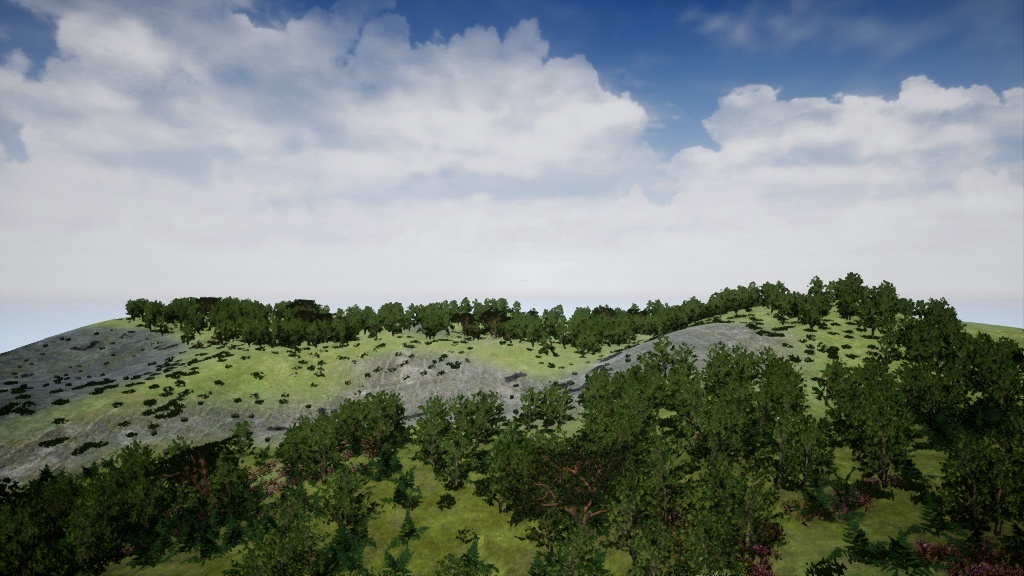
\includegraphics[width=.27\linewidth]{images/airsim_thresh/img_1.jpg} &
    % 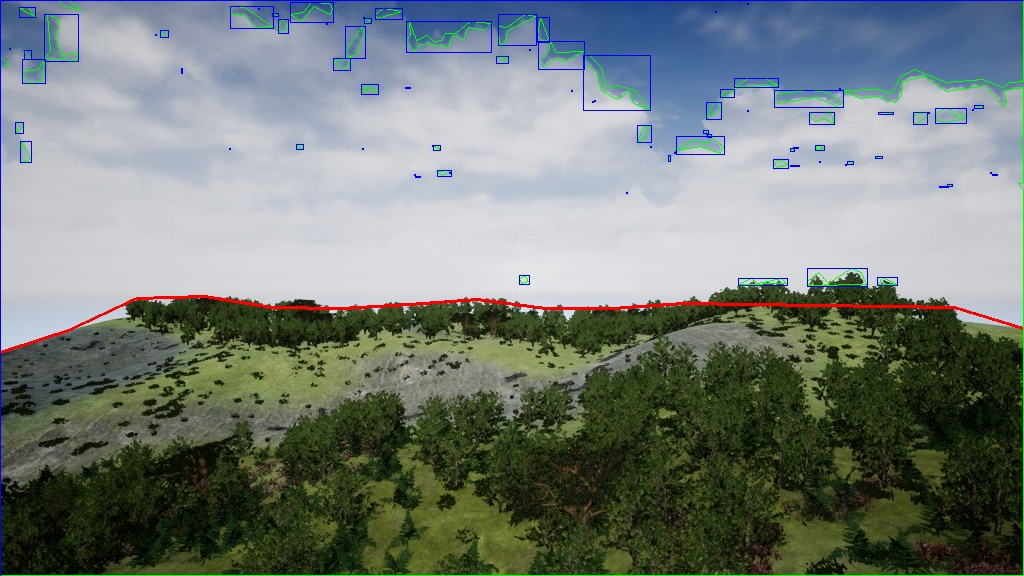
\includegraphics[width=.27\linewidth]{images/airsim_thresh/img_adaptive_1.jpg} &
    % 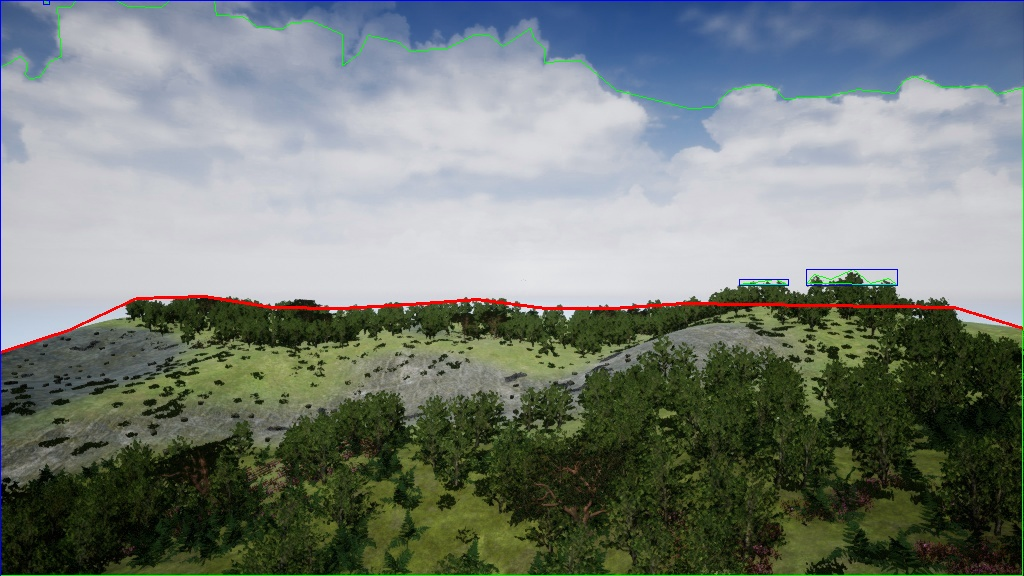
\includegraphics[width=.27\linewidth]{images/airsim_thresh/img_thresh_1.jpg} \\
    
    % 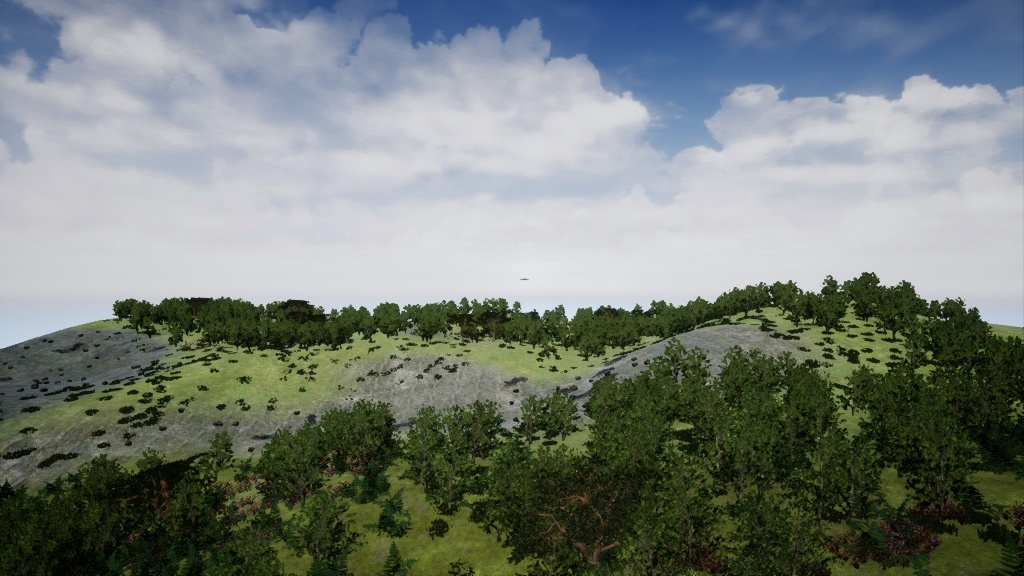
\includegraphics[width=.27\linewidth]{images/airsim_thresh/img_2.jpg} &
    % 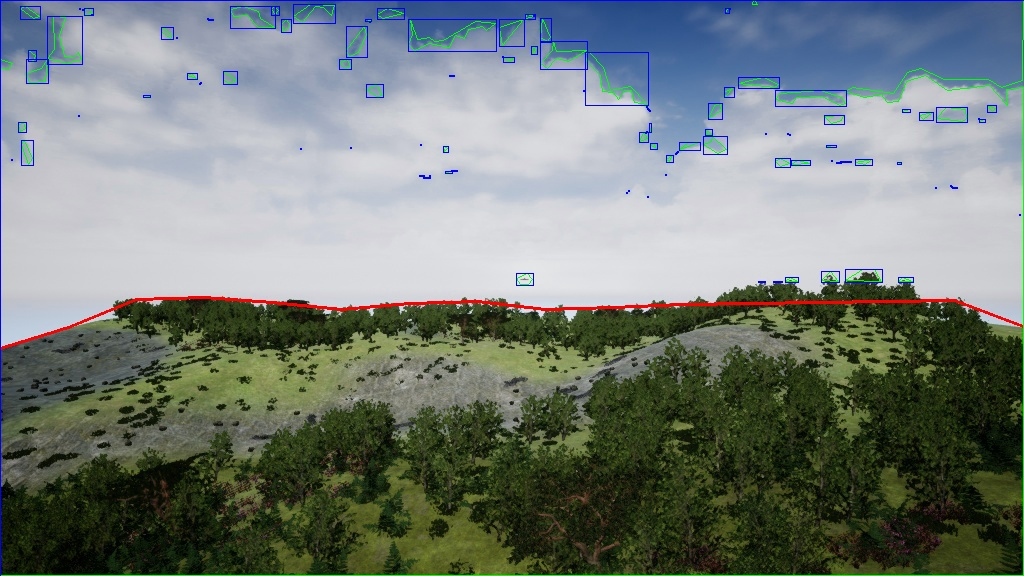
\includegraphics[width=.27\linewidth]{images/airsim_thresh/img_adaptive_2.jpg} &
    % 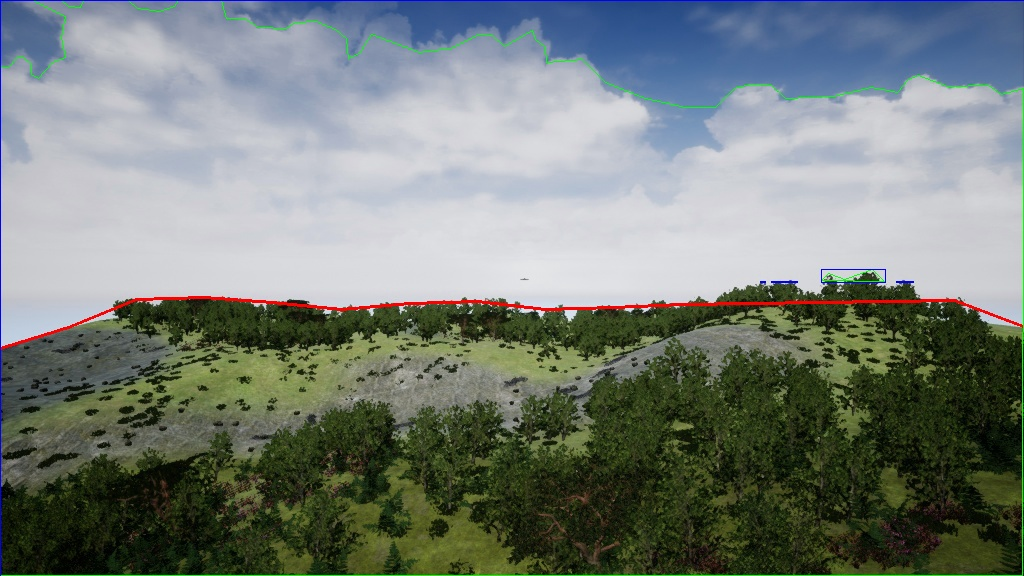
\includegraphics[width=.27\linewidth]{images/airsim_thresh/img_thresh_2.jpg} \\
    
    % 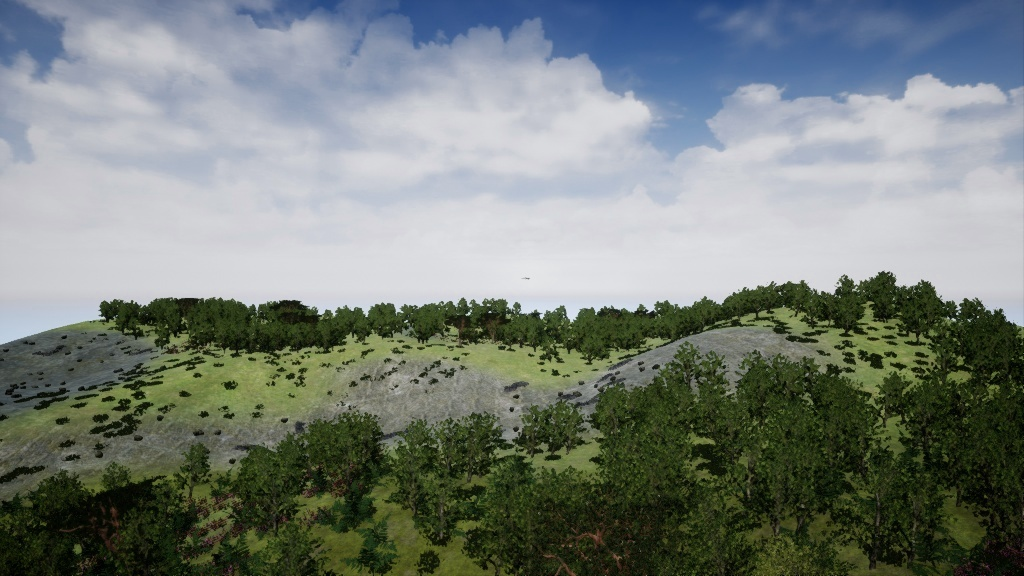
\includegraphics[width=.27\linewidth]{images/airsim_thresh/img_3.jpg} &
    % 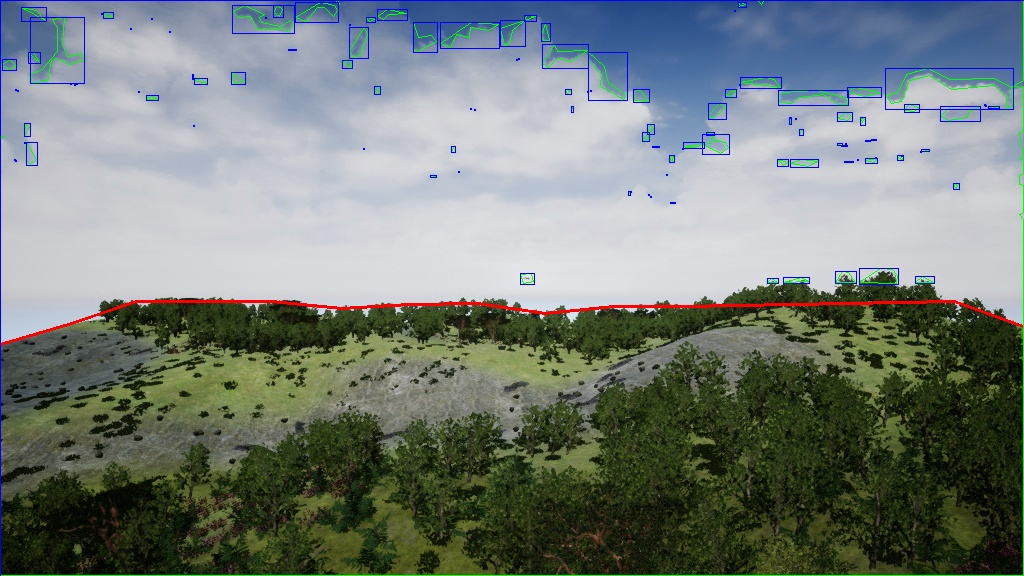
\includegraphics[width=.27\linewidth]{images/airsim_thresh/img_adaptive_3.jpg} &
    % 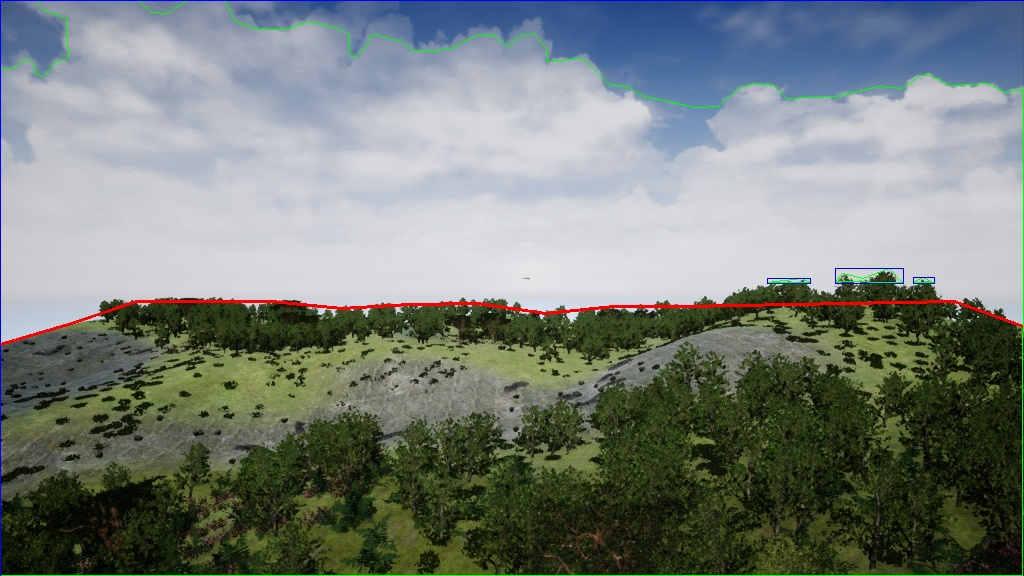
\includegraphics[width=.27\linewidth]{images/airsim_thresh/img_thresh_3.jpg} \\
    
    % 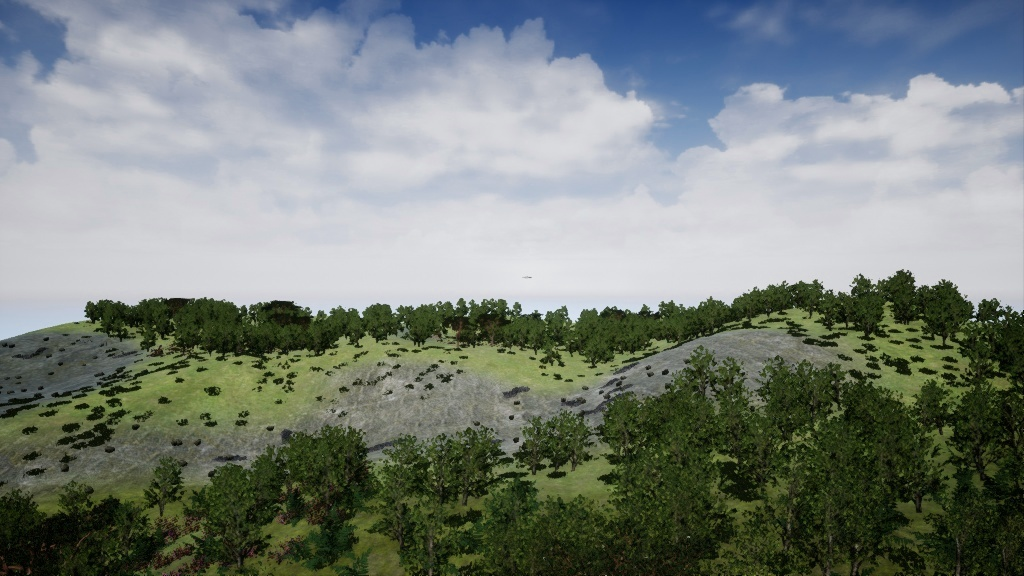
\includegraphics[width=.27\linewidth]{images/airsim_thresh/img_4.jpg} &
    % 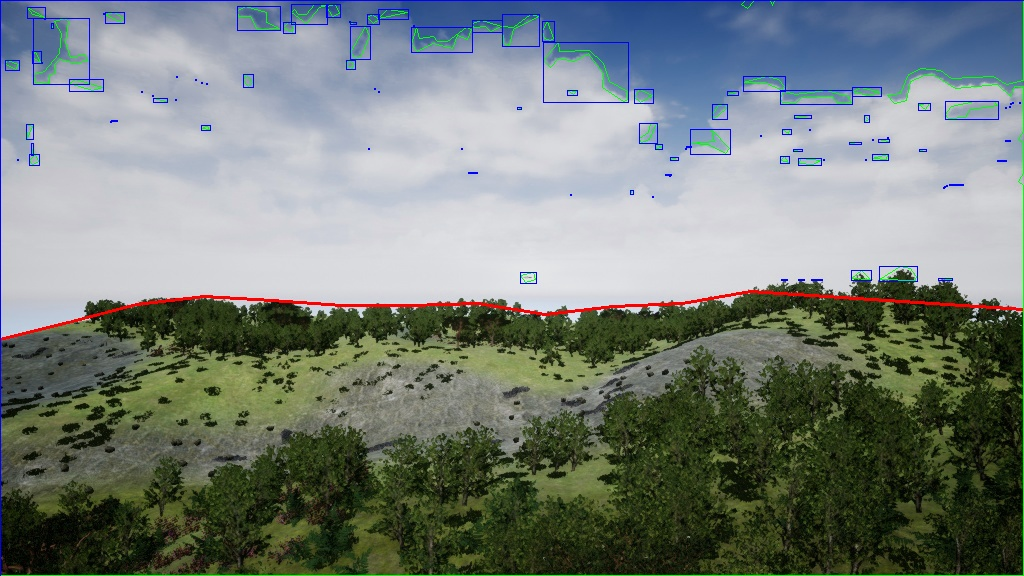
\includegraphics[width=.27\linewidth]{images/airsim_thresh/img_adaptive_4.jpg} &
    % 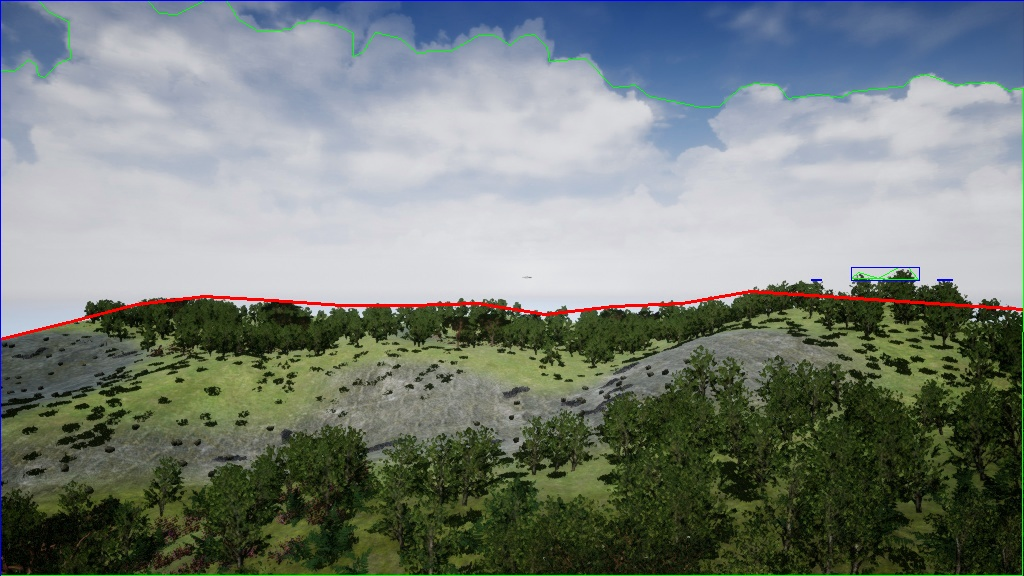
\includegraphics[width=.27\linewidth]{images/airsim_thresh/img_thresh_4.jpg} \\
    
    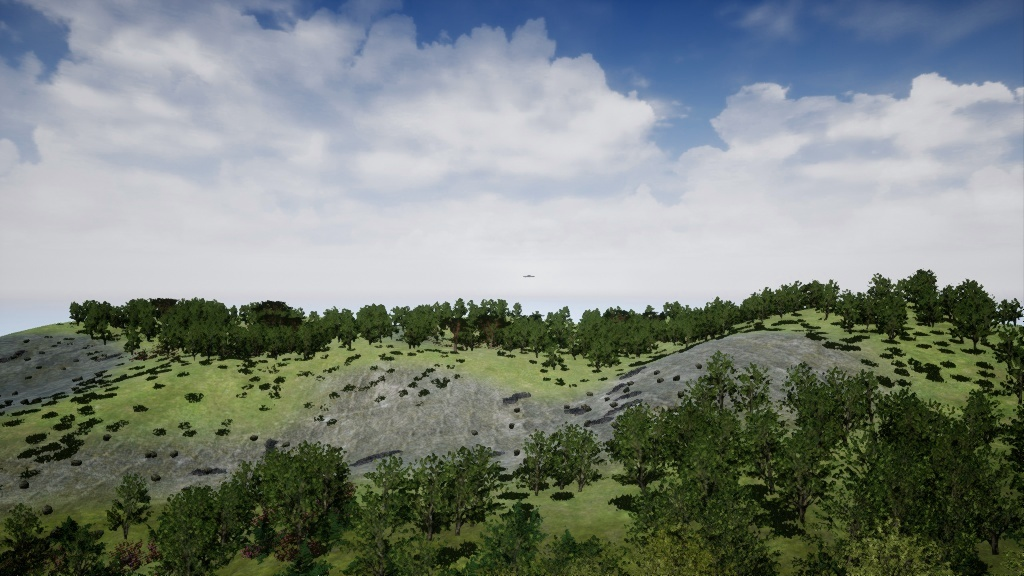
\includegraphics[width=.27\linewidth]{images/airsim_thresh/img_5.jpg} &
    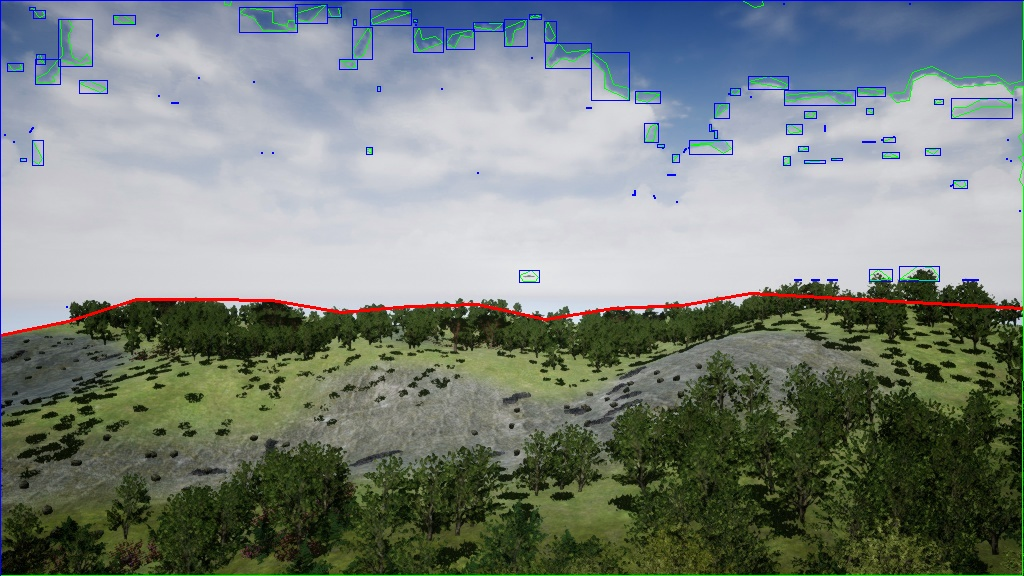
\includegraphics[width=.27\linewidth]{images/airsim_thresh/img_adaptive_5.jpg} &
    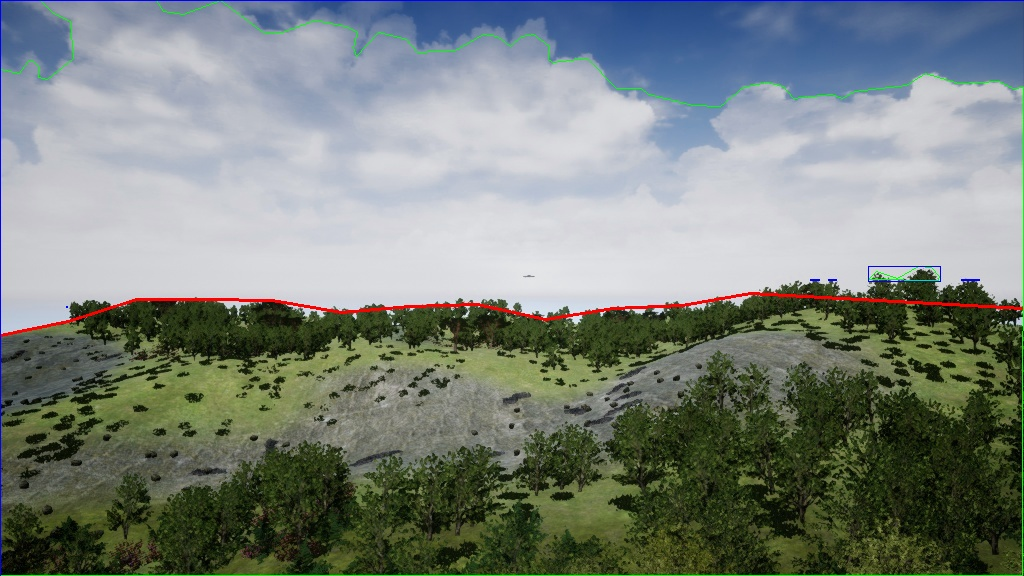
\includegraphics[width=.27\linewidth]{images/airsim_thresh/img_thresh_5.jpg} \\
    
    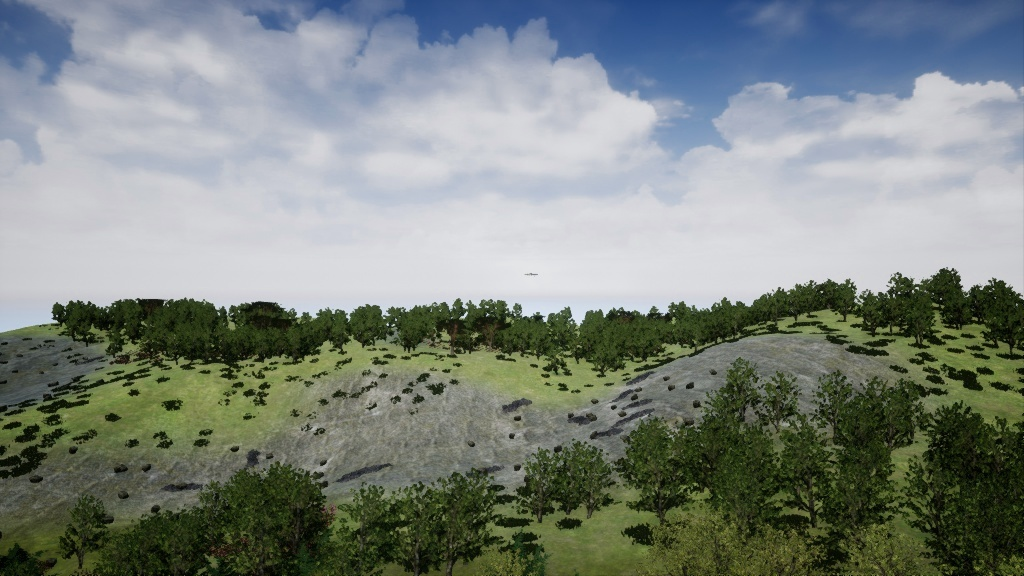
\includegraphics[width=.27\linewidth]{images/airsim_thresh/img_6.jpg} &
    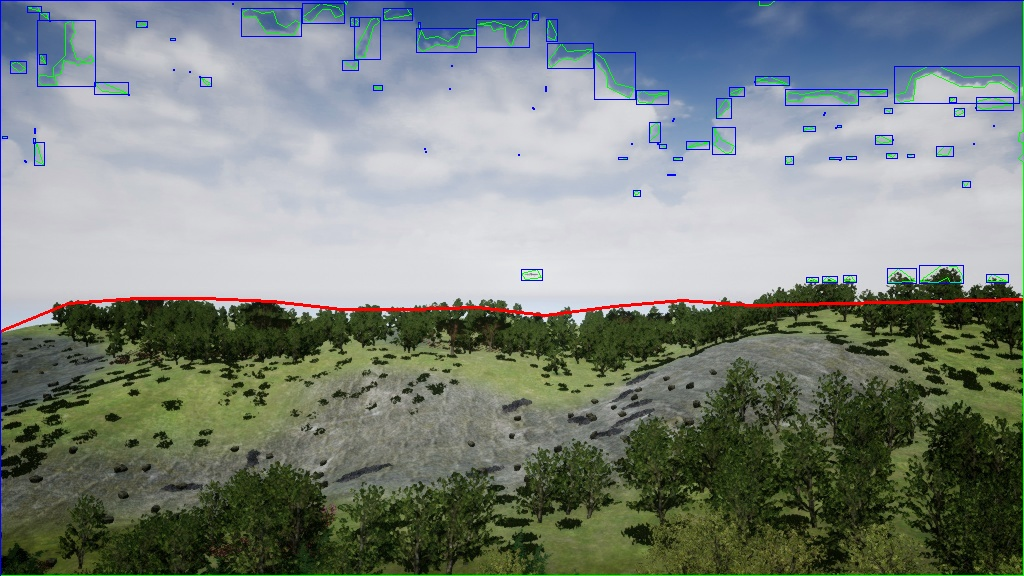
\includegraphics[width=.27\linewidth]{images/airsim_thresh/img_adaptive_6.jpg} &
    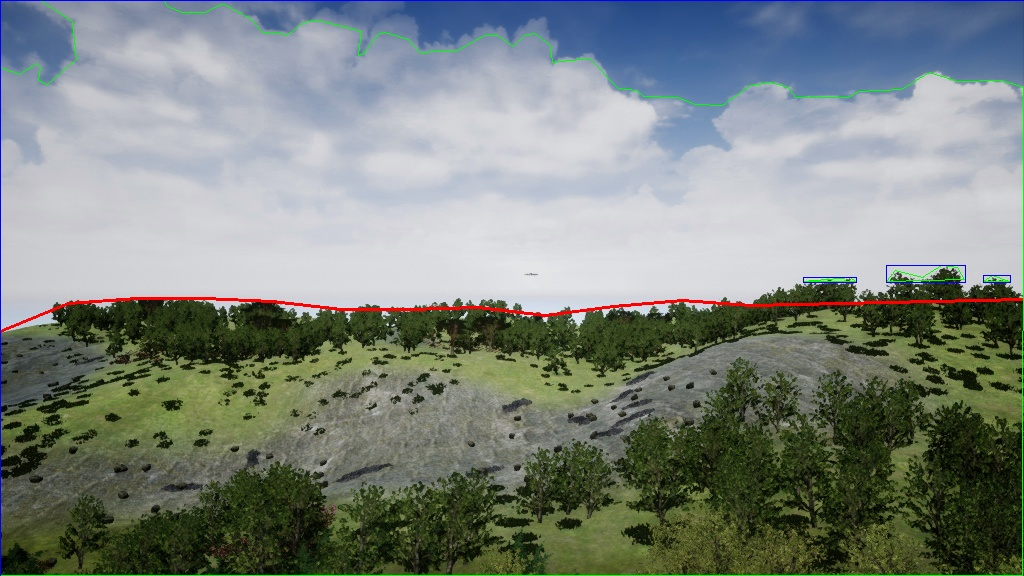
\includegraphics[width=.27\linewidth]{images/airsim_thresh/img_thresh_6.jpg} \\
    
    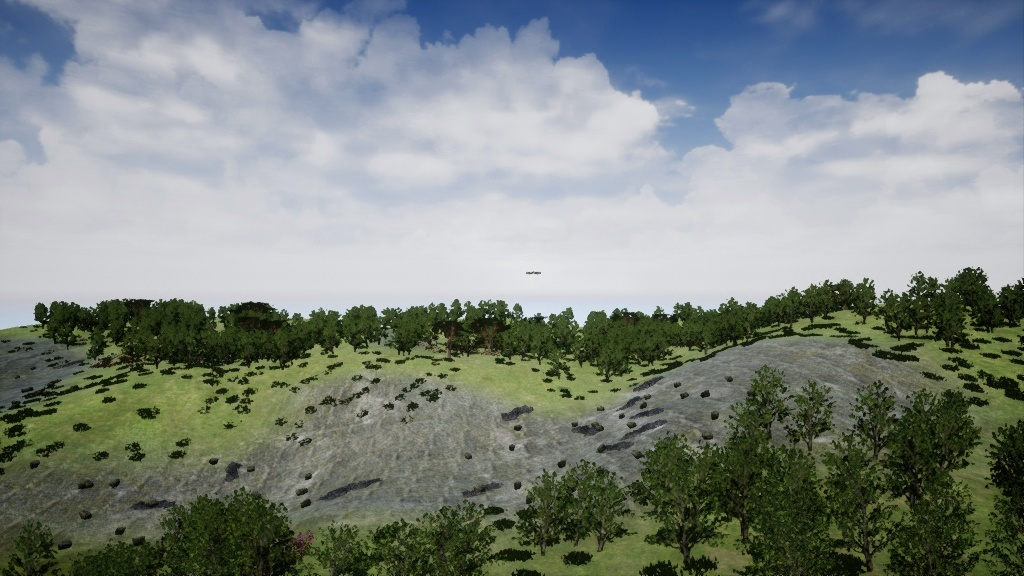
\includegraphics[width=.27\linewidth]{images/airsim_thresh/img_7.jpg} &
    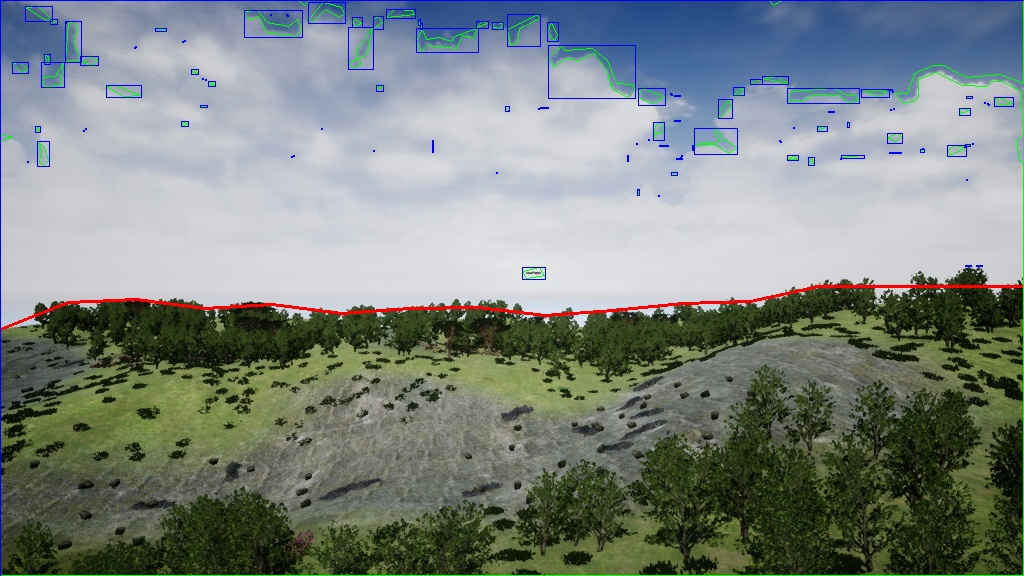
\includegraphics[width=.27\linewidth]{images/airsim_thresh/img_adaptive_7.jpg} &
    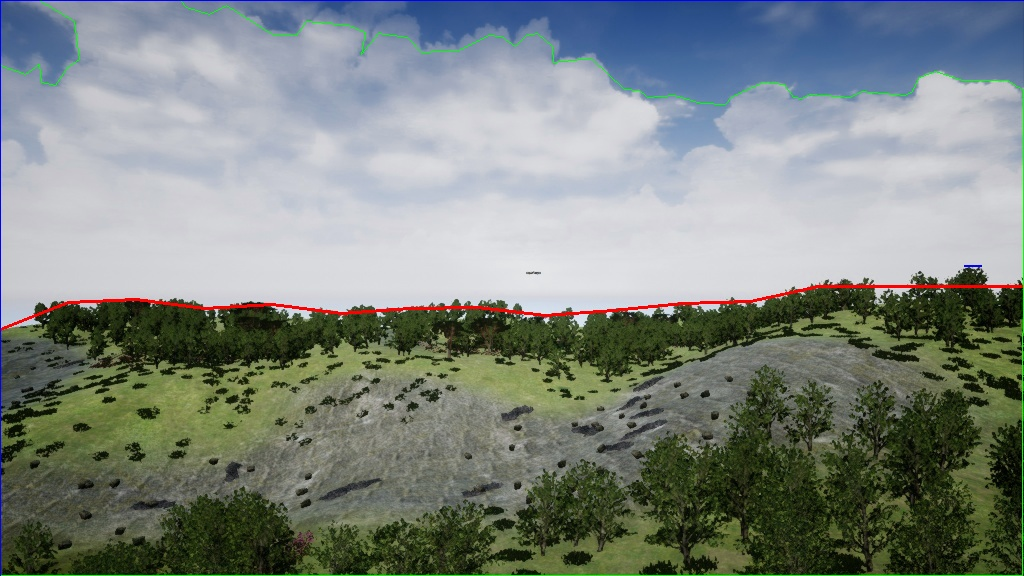
\includegraphics[width=.27\linewidth]{images/airsim_thresh/img_thresh_7.jpg} \\
    
    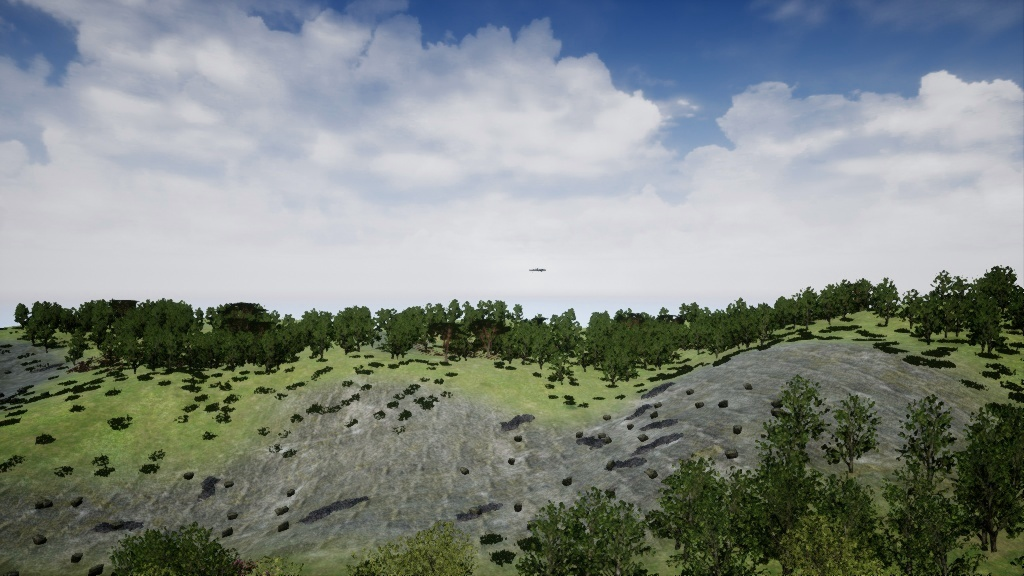
\includegraphics[width=.27\linewidth]{images/airsim_thresh/img_8.jpg} &
    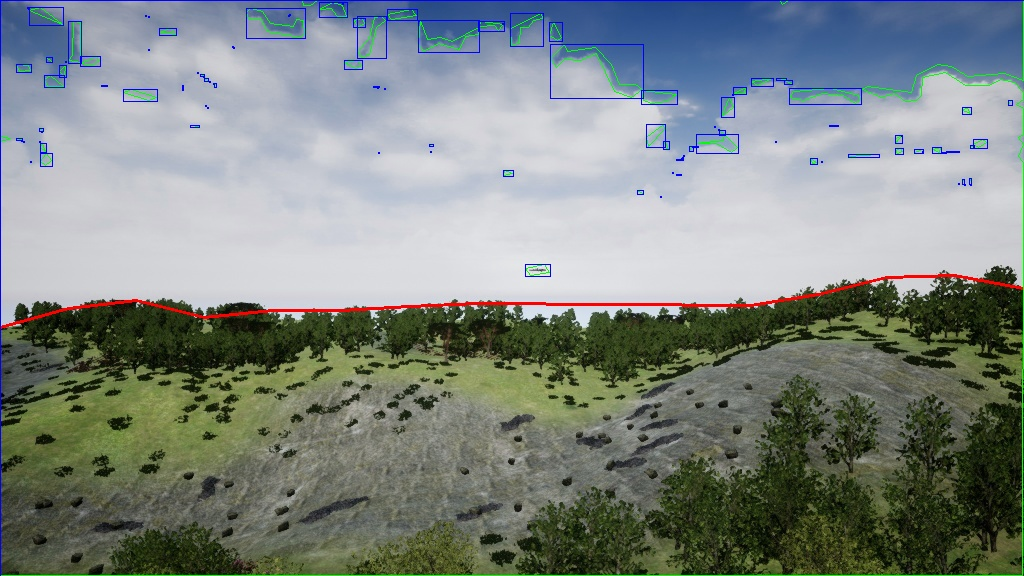
\includegraphics[width=.27\linewidth]{images/airsim_thresh/img_adaptive_8.jpg} &
    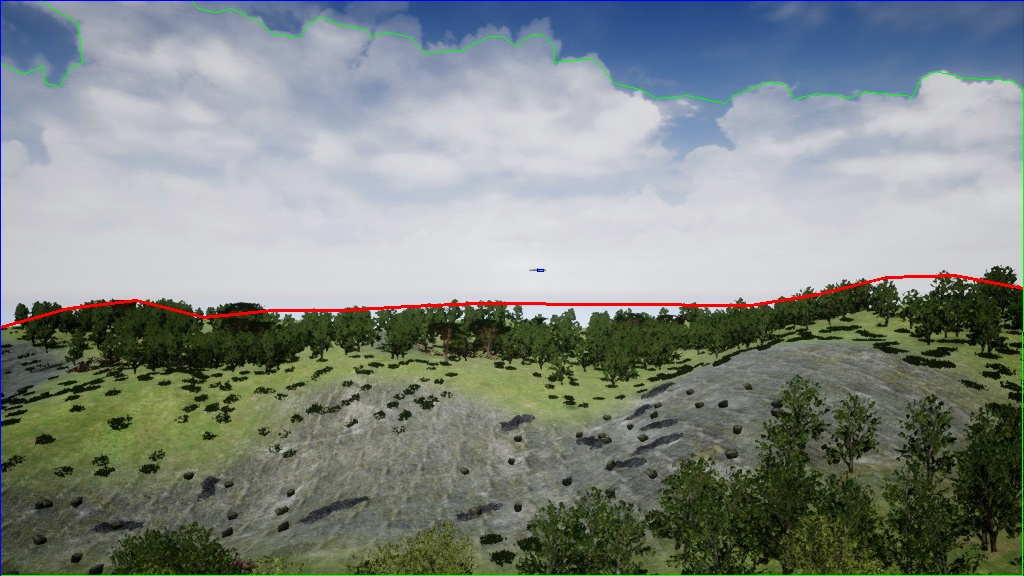
\includegraphics[width=.27\linewidth]{images/airsim_thresh/img_thresh_8.jpg} \\
    
    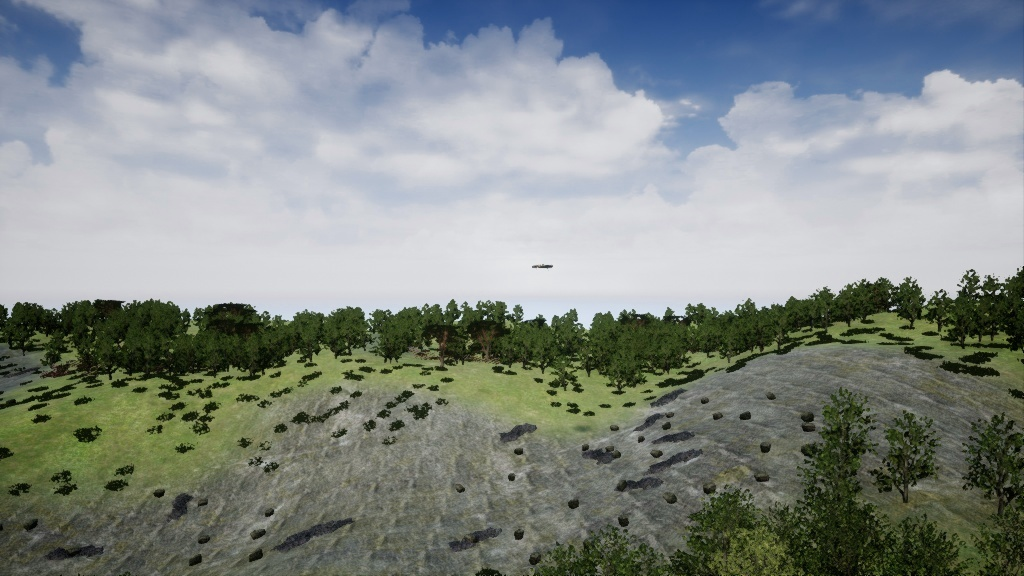
\includegraphics[width=.27\linewidth]{images/airsim_thresh/img_9.jpg} &
    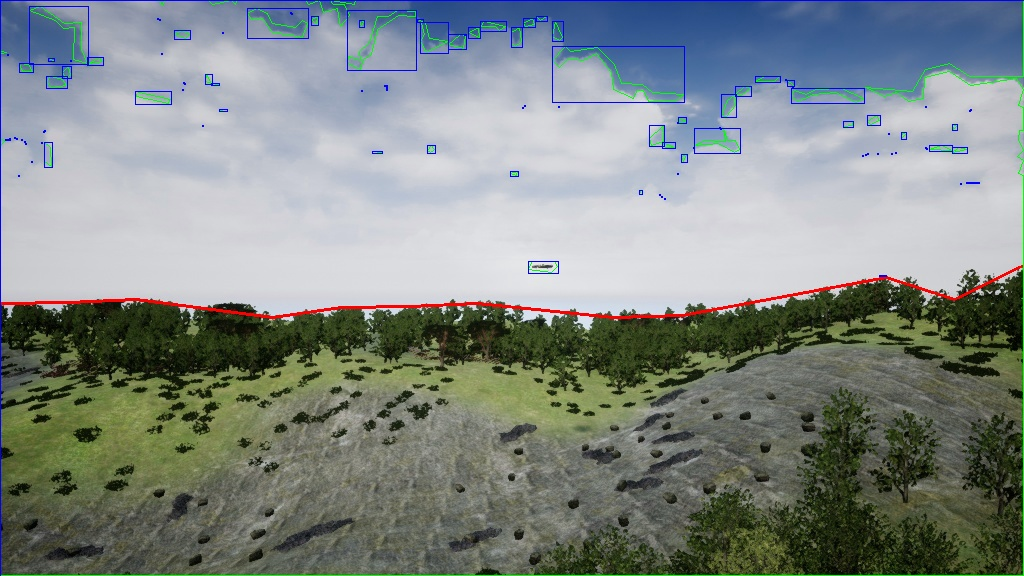
\includegraphics[width=.27\linewidth]{images/airsim_thresh/img_adaptive_9.jpg} &
    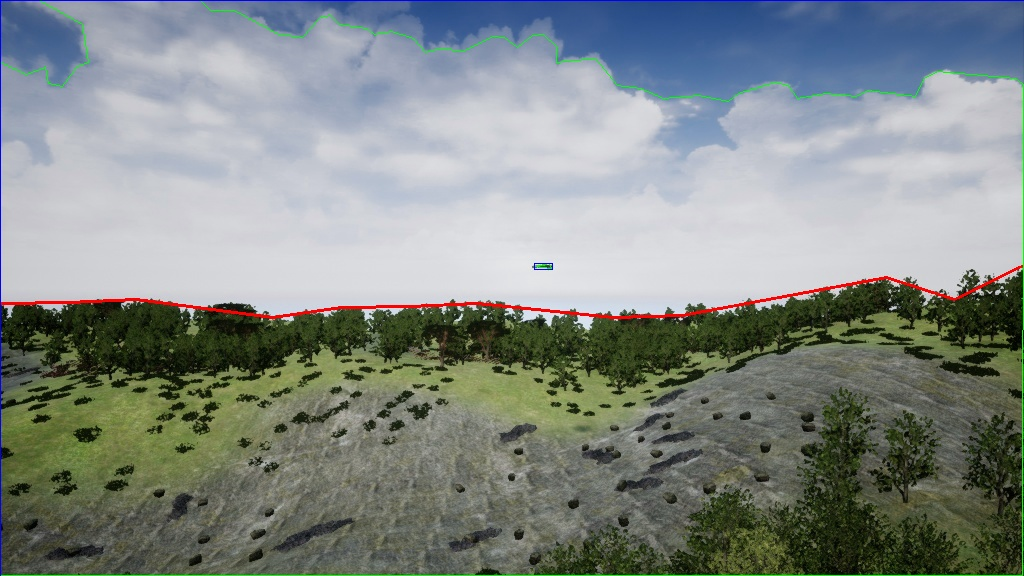
\includegraphics[width=.27\linewidth]{images/airsim_thresh/img_thresh_9.jpg} \\
    
    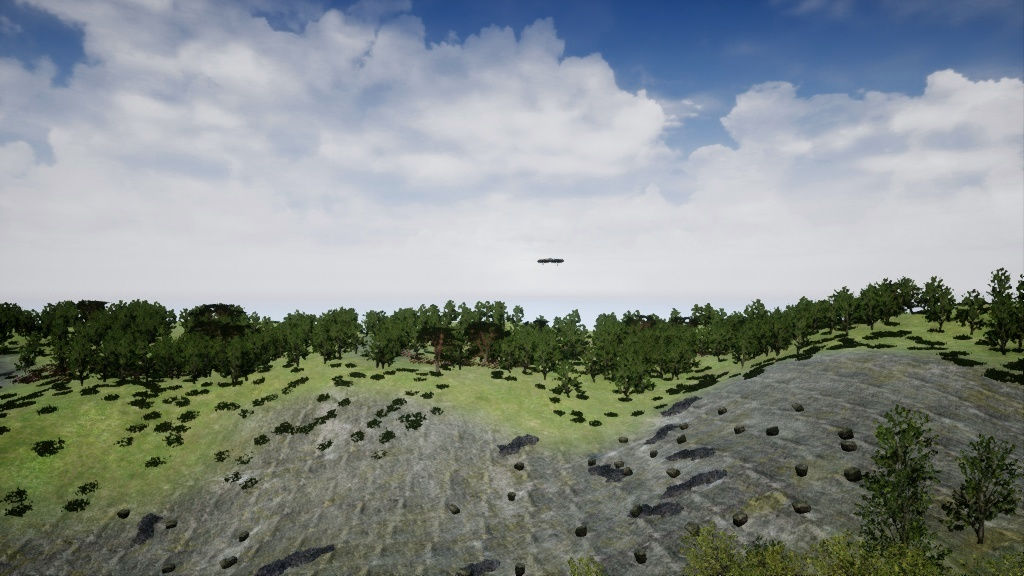
\includegraphics[width=.27\linewidth]{images/airsim_thresh/img_10.jpg} &
    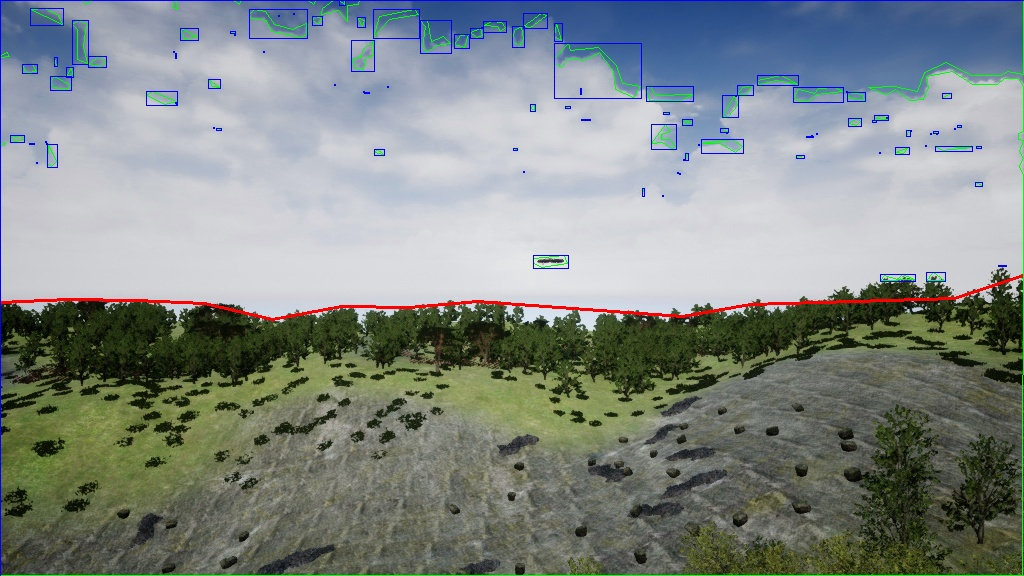
\includegraphics[width=.27\linewidth]{images/airsim_thresh/img_adaptive_10.jpg} &
    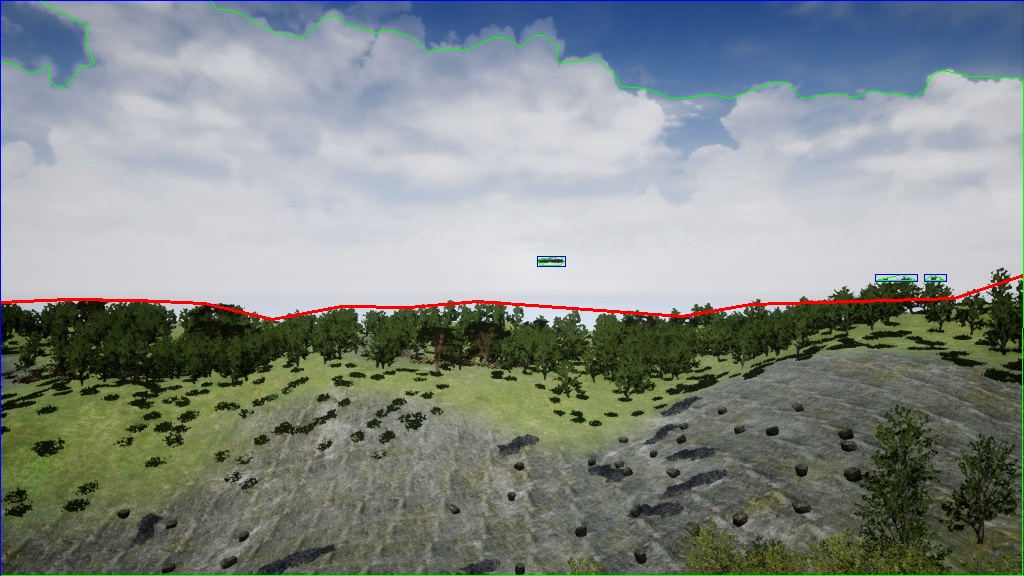
\includegraphics[width=.27\linewidth]{images/airsim_thresh/img_thresh_10.jpg} \\
    
    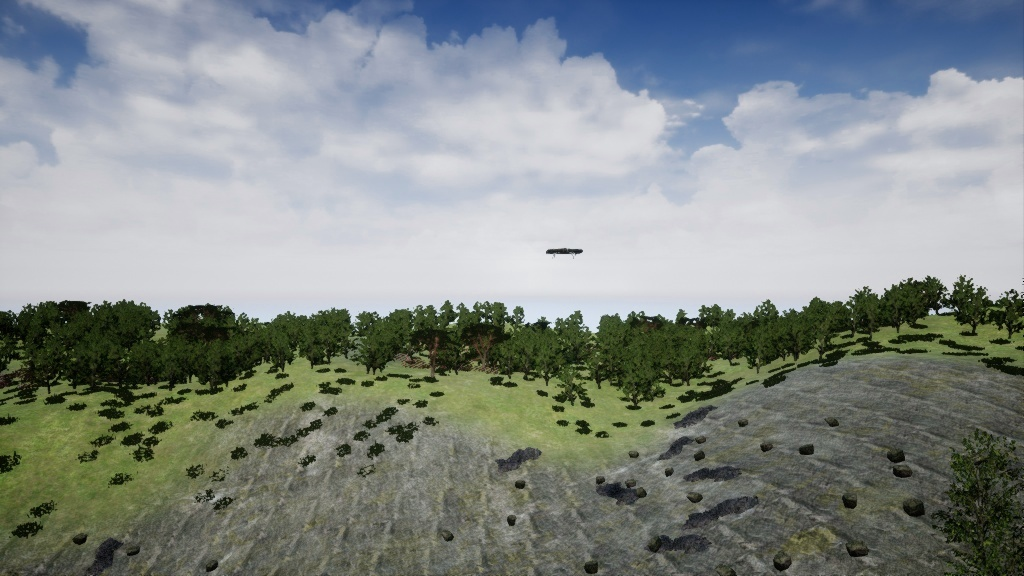
\includegraphics[width=.27\linewidth]{images/airsim_thresh/img_11.jpg} &
    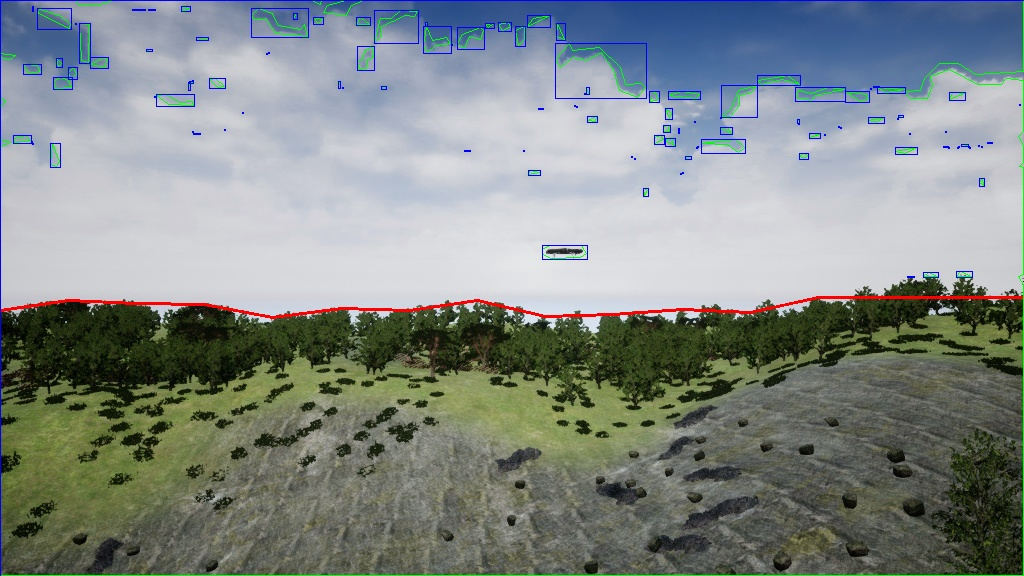
\includegraphics[width=.27\linewidth]{images/airsim_thresh/img_adaptive_11.jpg} &
    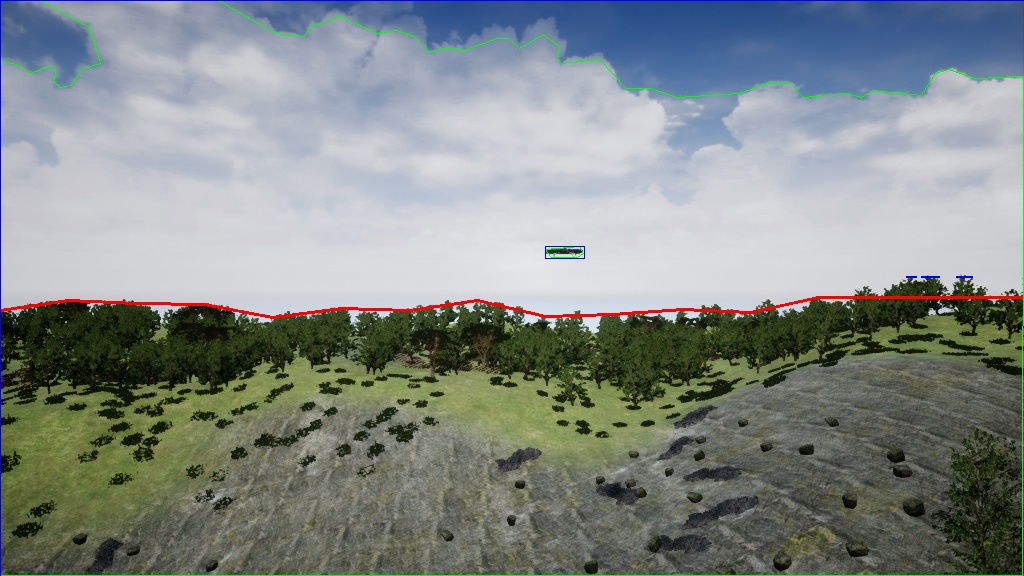
\includegraphics[width=.27\linewidth]{images/airsim_thresh/img_thresh_11.jpg} \\
    
    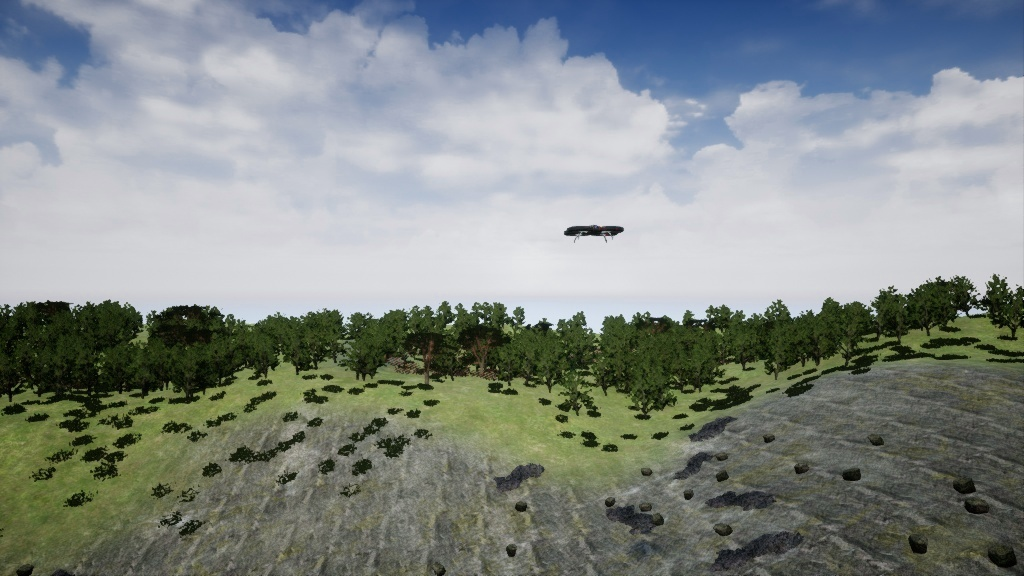
\includegraphics[width=.27\linewidth]{images/airsim_thresh/img_12.jpg} &
    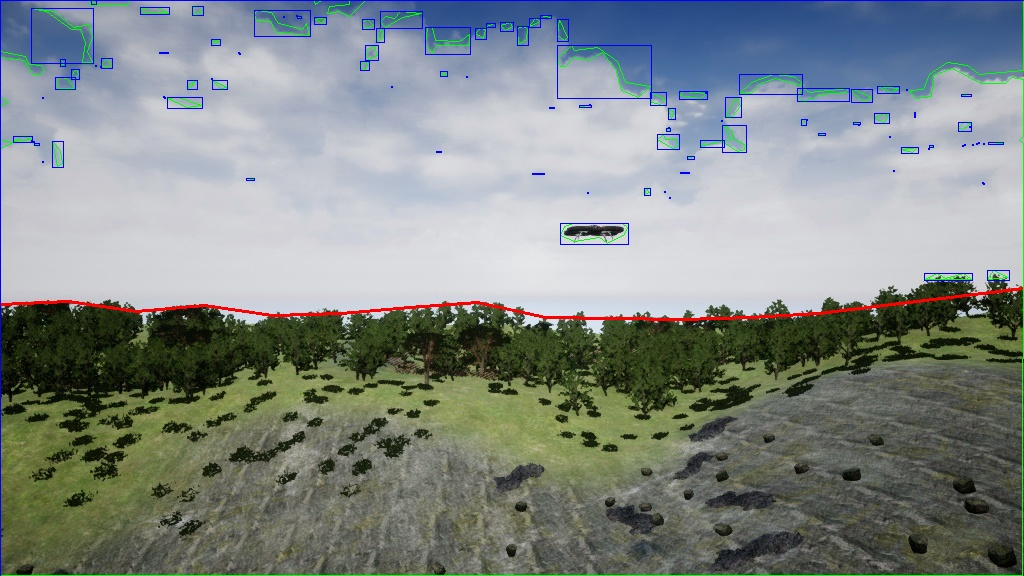
\includegraphics[width=.27\linewidth]{images/airsim_thresh/img_adaptive_12.jpg} &
    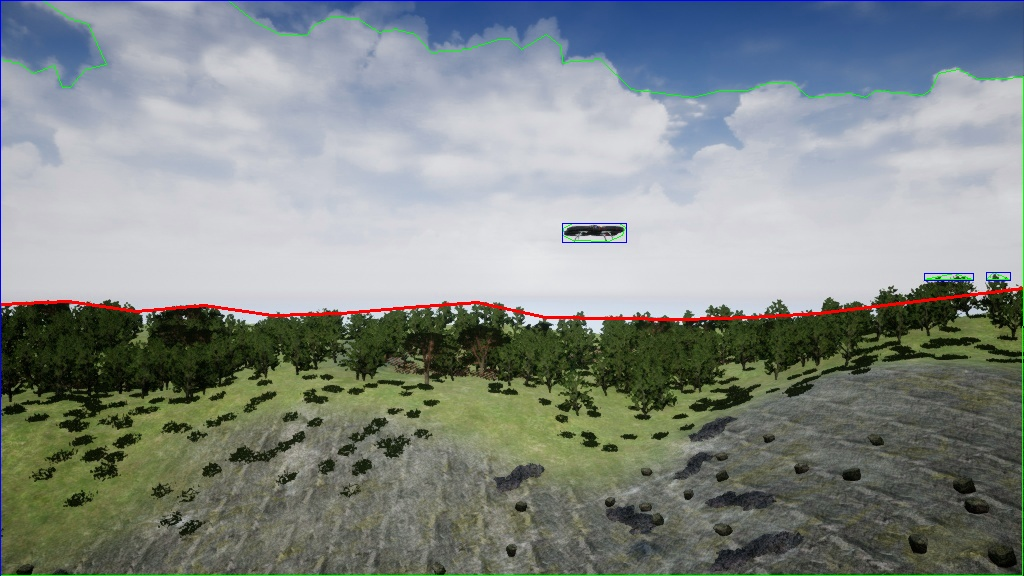
\includegraphics[width=.27\linewidth]{images/airsim_thresh/img_thresh_12.jpg} \\
    
    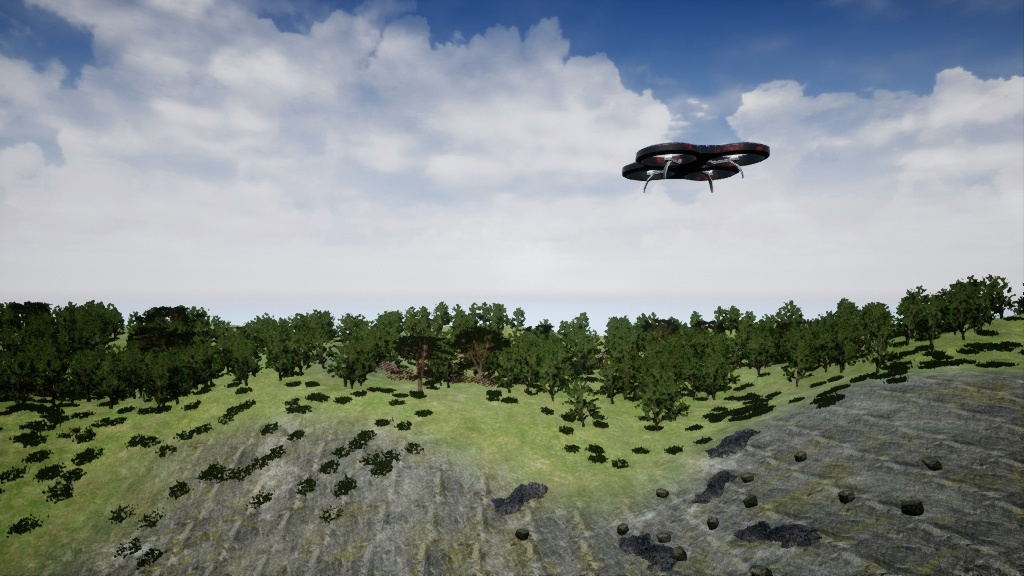
\includegraphics[width=.27\linewidth]{images/airsim_thresh/img_13.jpg} &
    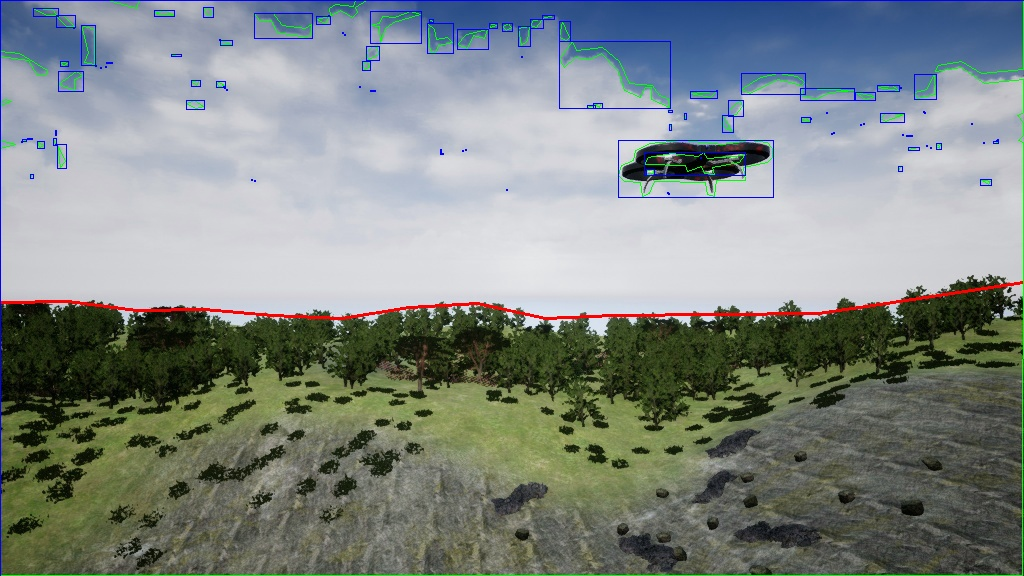
\includegraphics[width=.27\linewidth]{images/airsim_thresh/img_adaptive_13.jpg} &
    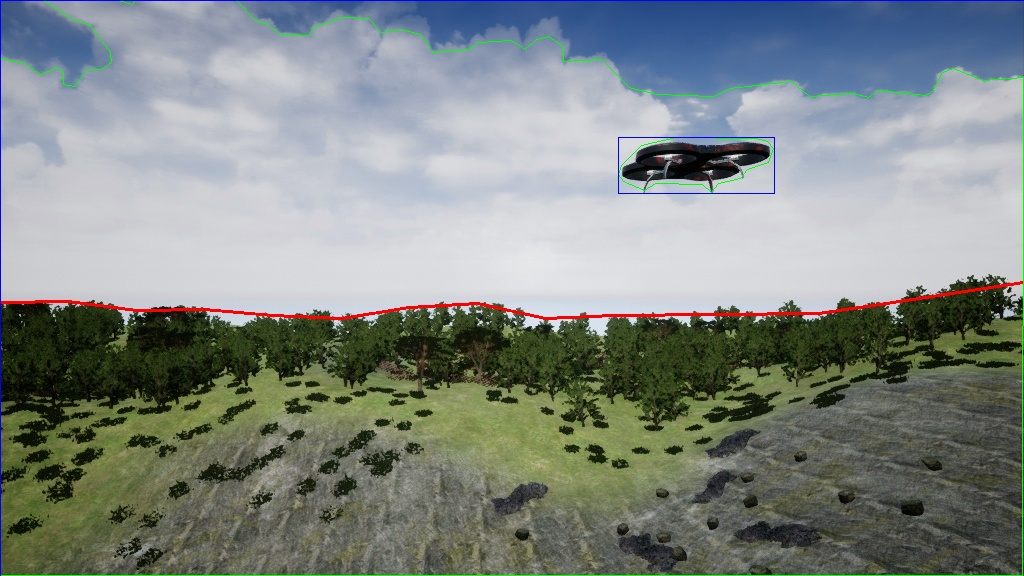
\includegraphics[width=.27\linewidth]{images/airsim_thresh/img_thresh_13.jpg} \\
    \end{tabular}
    \caption{Comparition of threshold and adaptive-threshold}
    \label{fig:thresh_compar}
\end{figure}

The preprocessing function takes an OpenCV image.
At first, it detects the horizon.
For this, it takes a series of numbers (line 2).
These points become the inflexion point of the segmented line of the horizon borderline.
Based on the complexity of the horizon (how segmented the line should be) not all the points are used.
After applying the horizon detect, comes the image processing part in question.
There is a series of OpenCV functions applied to the image (line 49-54).
There is an adaptive threshold function is replaced by a regular threshold function.
This was a necessity due the xfOpenCV does not have the adaptive threshold function implemented.
For the final result, both functions provide similar results, thus the two functions are interchangeable (\cref{fig:thresh_compar}).
There was also an attempt to implement the adaptive threshold for FPGA, but at the validation, the error measure was usually over 1\% which is too high error rate for an image processing system.
The final step is to find the contours on the image.
However, this part cannot be included in the FPGA system since there is a double cycle that manipulates the image, thus ruining the dataflow.

\section{HLS Prepocess} % 3401 characters

The implemented solution of the preprocessing block is the same as in the python block.
In C however, there must be temporary storage to be specified (line 17,21,23,29)
These variables later will be optimised according to the directives.
There can be seen temporarily removed lines that are corresponding with the Otsu threshold, and the adaptive threshold implementations.
The Otsu method was removed due to dataflow optimizations, but the threshold value is set according to offline Otsu calculations.
The adaptive threshold had too much error, hence it ruined the otherwise proper algorithm.
The other interesting part of this code is the streaming interface, and the \codeword{xf::Mat} conversation.
To transfer data to the FPGA, an AXI interface must be used.
The synthesis is not able to convert a struct or class to AXI data, thus other means of data transfer should be implemented.
The easiest is to transfer an array of data, which is a convenient solution, however, due to type conversations (change between OpenCV pixel type, AXI type, and xcOpenCV type) this solution was not feasible.
The other solution which requires more work and programming is to transfer the data through a stream.
For this, the VDMA is required.
The HLS generated IP has to be connected to the ZYNQ subsystem and the VDMA in and out streaming ports.
The system after uploading the preprocess block with the required kernels (all kernels require a separate kernel port to keep the dataflow) and sizes, the VDMA can be started as well.
The memory addresses should be set, for the python program to save the image to the read address offset of the VDMA.
The VDMA than creates a stream of the memory and transfers the data to the preprocessing.
The output of the preprocess sends the data back to the VDMA, that saves that data to a separate place on the memory.
the python system can read the memory and continue, with the processed image.
The uploading of the boxes can be done before the system start but the image load and write must be waited for.
This plus the latency of the system can cause async execution of the code.
This has to be handled by the python program as well.

\begin{figure}
    \centering
    
\includegraphics[width=.32\linewidth]{images/preproc/out_ocv.jpg}
    \includegraphics[width=.32\linewidth]{images/preproc/hls_out.jpg}
    % \includegraphics[width=.32\linewidth]{images/preproc/error.png}
    % \includegraphics[width=.32\linewidth]{images/preproc/out_ocv_negative.jpg}
    % \includegraphics[width=.32\linewidth]{images/preproc/hls_out_negative.jpg}
    \includegraphics[width=.32\linewidth]{images/preproc/error_negative.png}
    \caption{Preprocessing comparison of the OpenCV image, the HLS block, and the differences. The error image are negative for better comparison.}
    \label{fig:preproc_compare}
\end{figure}

To validate the software, a test bench source (\cref{code:test_bench}) was made.
This source is also required by the Synthesis and the simulation processes of the HLS.
In this program, the same image is processed by both the original OpenCV and the HLS block as well.
The HLS block is a simulated process, which means that the computer tries to replicate the effect of the directives in an SI processor.
This requires a lot of time, and resource, and also in some cases (eg. loading in a FIFO) not even possible to implement.
The HLS tries to calculate the parameters of the hardware and compares it to the results of the simulated run.
If the values are correct the original and the hardware implementation results are compared (line 36-56).
To have a reference to compare, a series of OpenCV function was introduced to the test bench (line 13-18).
These functions are the C implementations instead of the python, which is used in the algorithm, but the underlying logic is the same.
The OpenCV installed on the computer is also compiled in release more, hence the functionalities are all optimised.
After the reference image, the data is converted to a \codeword{hls::stream} (line 24), for easier transfer.
The stream is fed to the block and the output stream is written back to another image (line 28).
After the results are written in two variable, by both the OpenCV and the HLS block as well, the difference between the two is calculated (line 32).
The test showed an average of 0.15\%of pixels above the error threshold.
Here a simple differential calculation is used, but in some cases, other error measures had to be introduced.
All three image is written to the disc for visual comparison (line 20,30,34) (\cref{fig:preproc_compare}).

The final system and the HLS implementation results can be seen in \cref{tab:preproc_hls_usage}.
The minimal and the maximal latency is between 8321540 and 8331485, where the greatest contributor is the Gaussian Blur and the Threshold (\cref{tab:preproc_hls_latency}).
After adding the connectivity and the VDMA to the design file, the system utilization got a little higher (\cref{tab:preproc_final_usage}).

\begin{table}
    \centering
    \caption{Preprocessing HLS block hardware requirements}
    \label{tab:preproc_hls_usage}
    \begin{tabular}{|l|l|l|l|l|l|}
    \hline
    Name &  BRAM\_18K &  DSP48E &  FF &  LUT &  URAM \\ \hline
    DSP & - & - & - & - & - \\ \hline
    Expression & - & - & 0 & 71 & - \\ \hline
    FIFO & 0 & - & 171 & 1316 & - \\ \hline
    Instance & 46 & 4 & 7617 & 13636 & - \\ \hline
    Memory & - & - & - & - & - \\ \hline
    Multiplexer & - & - & - & 90 & - \\ \hline
    Register & - & - & 15 & - & - \\ \hline
    Total & 46 & 4 & 7803 & 15113 & 0 \\ \hline
    Available & 1824 & 2520 & 548160 & 274080 & 0 \\ \hline
    Utilization (\%) & 2 & $\approx$ 0 & 1 & 5 & 0 \\ \hline
    \end{tabular}
\end{table}

\begin{table}
    \centering
    \caption{Latency measurements of the main components on the Preprocess block}
    \label{tab:preproc_hls_latency}
    \begin{tabular}{|l|c|c|c|c|}
    \hline
    Module & Latency & & Interval \\ \hline
    & min &  max &  min &  max \\ \hline
    erode90 & 105 & 8331455 & 105 & 8331455 \\ \hline
    erode & 105 & 8331455 & 105 & 8331455 \\ \hline
    dilate & 105 & 8331455 & 105 & 8331455 \\ \hline
    GaussianBlur & 8321526 & 8321526 & 8321526 & 8321526  \\ \hline
    xfMat2AXIvideo & 1 & 8303041 & 1 & 8303041 \\ \hline
    AXIvideo2xfMat & 3 & 8305203 & 3 & 8305203 \\ \hline
    Threshold & 8300881 & 8300881 & 8300881 & 8300881 \\ \hline
    \end{tabular}
\end{table}

% \begin{table}
% \centering
% \caption{Clocking results for the Preprocess block}
% \label{tab:preproc_hls_timing}
% \begin{tabular}{|l|l|}
% \hline
% \end{tabular}
% \end{table}

\begin{table}
\centering
\caption{Final preprocess Overlay utilization table}
\label{tab:preproc_final_usage}
\begin{tabular}{|l|l|l|l|}
\hline
Resource & Utilization & Available & Utilization \% \\ \hline
LUT & 15725 & 274080 & 5.74 \\ \hline
LUTRAM & 2674 & 144000 & 1.86 \\ \hline
FF & 20511 & 548160 & 3.74 \\ \hline
BRAM & 34 & 912 & 3.73 \\ \hline
DSP & 4 & 2520 & 0.16 \\ \hline
BUFG & 1 & 404 & 0.25 \\ \hline
\end{tabular}
\end{table}

\begin{figure}
    \centering
    \includegraphics{images/power_report.png}
    \caption{Power requirements of the final hardware}
    \label{fig:power}
\end{figure}

\clearpage

\section{Adaptive Threshold} % 1670 characters
The adaptive threshold function is one of the used OpenCV function of the avoid algorithm.
This function, however, is not implemented in the xfOpenCV library, hence it has been replicated according to the OpenCV implementation.
For this, another HLS block was created (\cref{code:adaptive_thrash}).
The first approach was to modify the custom convolution implementation of the xfOpenCV.
This required to remove the kernel input of the function and add a division at the end of the kernel function.
The resulting algorithm did not satisfy the correctness criteria of error measure beeing under 1\%.
The function also required to use of a modified function of an already validated one.
This makes the further development hard, and the maintenance of the current code a nightmare.
After studying the code of the original OpenCV implementation, the obvious solution became clear.
In the Original library, the Adaptive threshold is not implemented with a dedicated function, but a box filter chained with a decision logic.
By chaining this two logic the end result seemed to be satisfied until the function was not connected to other functions.
As it turns out the error measure at the validation of the boxFilter solution in the xfOpenCV library is not set up for matching the original exactly but allows the values to jitter by 1 (\cref{code:box_error}).
At first, it can not be seen on the image, but when multiple functions are applied to the output of the boxFilters this error can result in a huge difference.

\lstset{
    language=C,
    caption={Error measure of the Boxfilter algorithm in the xfOpenCV library},
    label={code:box_error},
    keywordstyle=\color{red},
    stringstyle=\color{blue},
    commentstyle=\color{green},
    morecomment=[l][\color{magenta}]{\#},
    columns=fullflexible,
    breaklines=true,
    postbreak=\mbox{\textcolor{red}{$\hookrightarrow$}\space},
}
\begin{lstlisting}
double minval=256,maxval=0;
	int cnt = 0;
	for (int i=0;i<in_img.rows;i++)
	{
		for(int j=0;j<in_img.cols;j++)
		{
			uchar v = diff.at<uchar>(i,j);
			if (v>1)
				cnt++;
			if (minval > v )
				minval = v;
			if (maxval < v)
				maxval = v;
		}
	}
	float err_per = 100.0*(float)cnt/(in_img.rows*in_img.cols);
\end{lstlisting}

\begin{figure}[b]
    \centering
    \includegraphics[width=.32\linewidth]{images/box_filter/HLS_img.jpg}
    \includegraphics[width=.32\linewidth]{images/box_filter/diff_img.jpg}
    \includegraphics[width=.32\linewidth]{images/box_filter/OCV_img.jpg}
    \caption{The xfOpenCV boxFilter, the difference and the OpenCV boxFilter final result. The error is enhanced for better visual comparison}
    \label{fig:box_error}
\end{figure}

After correcting the error measure, the difference is still hardly noticeable, since it differs only by one, compared to a 256 long scale.
The error also has to be enhanced as well.
By introducing a special error measure (\cref{code:enhaced_box_error}), the visual similarities are clearly visible (\cref{fig:box_error}).
This measure displays white pixels where the two results are different exactly by one.
The error occurs only in one way, as every time the OpenCV implementation has larger values.
The cause expected to be a rounding error, however, no investigation is done in this topic.

\lstset{
    language=C,
    caption={Enhanced error measure of the Boxfilter},
    label={code:enhaced_box_error},
    keywordstyle=\color{red},
    stringstyle=\color{blue},
    commentstyle=\color{green},
    morecomment=[l][\color{magenta}]{\#},
    columns=fullflexible,
    breaklines=true,
    postbreak=\mbox{\textcolor{red}{$\hookrightarrow$}\space},
}
\begin{lstlisting}
for (int i=0;i<imgOutput.rows;i++){
	for(int j=0;j<imgOutput.cols;j++){
	if (ocv_thresh.at(i,j) == imgOutput.data[i*imgOutput.cols +j] + 1 ){
			diff.at<unsigned char>(i,j) = 255;
		}
		else{
			diff.at<unsigned char>(i,j) = 0;
		}
	}
}
\end{lstlisting}

\clearpage

\section{Start the Overlay} % 2070 characters
In the configuration file (\cref{code:preproc_start}), the overlay loaded through the PYNQ Overlay library.
This function requires the \codeword{.bit} file, and the \codeword{.hwh} to create the connections and the endpoints of the IPs (line 1-2).
The bit file contains the VDMA and the preprocess block as well.
There is a bug in the PYNQ system, about the interrupt signals of the ZYNQ processor subsystem.
Since the ZCU102 is not the main platform for the PYNQ the error is not expected to be solved soon.
To bypass this no interrupt signal should be connected to the ZYNQ in the block design.
However, for the Overlay function, all ports of every IP should be connected.
This includes the interrupt signals as well.
In the end, if both the VDMA and the ZYNQ block is to be used, the Overlays cannot be loaded properly.
The error in the python library, however, does not affect the FPGA code.
The blocks are working properly, without any disruption.
In the traditional workflow, after the generation of the bitstream, the C software should be written.
This case is not different, however here, the software is in python.
The VDMA control signals (lien 4-20) are described in the programming guide of the IP.
The settings of the IP and the addresses (line 22-27) can be set in the Vivado\texttrademark before the bitstream generation.
The image should be saved to a memory location, where the VDMA can read it.
For this, the memory should be allocated continuously (line 31,32,36).
After copying the image in place the preprocessing block can be started.
The preprocess block waits until the input stream does not provide enough data, hence starting this block first will keep the block waiting (line 53).
The write address offset \codeword{0x00} points to the control signals of the block, the \codeword{0x81} value starts the block.
The other \codeword{mmio} block is corresponding to the VDMA.
This block ha 2 port to set up, both in reading and writing side.
By providing the sufficient config data first the reading part is started (line 57-63).
After reading the image from the memory, and feeding it to the preprocess the write side is set up (line 69-73).
Finally, the \codeword{tmp} parameter reads the status of the IP.
Both IP is started and never stopped.
This means that every time the input image is always read by the VDMA.
If the image changed by the python program the VDMA starts to read the data in the next clock cycle.
If the image is not changed the previously loaded image is processed again.
With this, if the IPs are started the preprocessing block can load and read the data whenever it is best.

\section{Speed, Consumption} % 1461 characters

According to the previous tables (\cref{tab:preproc_hls_usage}, \cref{tab:preproc_hls_latency}), the IP block consumes 3.931 W energy.
The clock of the preprocess block is set to 5 ns speed and the resulting implementation finished with 1.226 ns WNS (Worst Negative Slack), 0.01 ns WHS (Worst Negative Slack) and 0.998 ns WPWS (Worst Pule Width Slack).
This adds up to $1.226 + 0.01 + 0.998 = 2.234 ns$ clock time.
Since it is way under the required 5 ns the implementation can easily run on 200 MHz clock.
The latency of the system is minimum 8,321,526 clock cycles, one frame is processed in $8,321,526 / (2\cdot10^8) = 41.608 ms$.
This makes it possible to process the input video around 24 fps $2\cdot10^8/8,321,526=24.034$. %($0.04160763 spf * 24 f = 0.99858312 s$).
This measurements are done for the template parameters \codeword{width=3840}, \codeword{height=2160} ($3840 * 2160 = 8,294,400 pixel$) UHD (Ultra-High-Definition) images.
The actual implementation, however, can be much faster than that, since the Gaussian blur and the Threshold functions are not that slow, as the synthesis shows.
The convolutional kernels are confusing the synthesiser, as the loops cannot be optimised in the compilation phase.
The synthesiser cannot determine the run count of the cycles, thus user-specified values must be given.
The User-specific values are computed by the maximal size of a possible image (the template parameters), but the function works according to the size of the loaded image.
As the resolution drops from UHD to FullHD, which was originally planned, the pixels to process drop down from 8,294,400 to 2,073,600.
The possible speed in this case $2,073,600 / (2\cdot10^8) = 10.368 ms$ and $2\cdot10^8/2,073,600 = 96.45$ fps.
With the $1024*576=589,824$ resolution of the airsim simulator, the possible speed is $589,824/ (2\cdot10^8) = 2.949 ms$ thus  $2\cdot10^8/589,824 = 339.084$ fps.
Both the 25 and the 96 fps are better result compared to the original 2.1 fps on the first run on the ZCU102.

\clearpage
\chapter{Summary} \label{ch:sum}

To use a Xilinx device, the Xilinx software should be used.
The first task was to get familiar with the workflow of an HLS hardware design.
This included the Vivado HLS, the Vivado and the PYNQ system as well.
To create a working hardware design the developer cannot rely just on the automated software functions but has to know the basic structure of the device.
Therefore the directives can be designed optimised.
The designer also has to know the exact working mechanism of the algorithm to implement.
The algorithms usually executed on a serial execution processor, and it affects the result as well.
For parallel execution, such as a hardware design, the code must be design, with the advantages and limitations of the hardware in mind.

The Xilinx xfOpenCV library was a great help in the development process since the library contains all the required functions.
After validating the required functions an acceleration block was established.
The block has to use dataflow to achieve maximal speed.
The steps of the algorithm are set up as in the original code.
The input of the block is a datastream of 8-bit unsigned data.
The incoming datastream is converted to a \codeword{xf::Mat} format.
For the convolution to work the block has to read in \codeword{kernel\_size-1} lines from the image.
This adds to the latency since every step waits until enough pixel is not present at the input side.
After converting the \codeword{xf:Mat} back to a stream the block feeds the stream to the outer program.
Since it is a streaming and dataflow system, the next image can be passed to the input right after the first, even the output image is not ready yet.
There are 3 functions (the two erode and the dilate) which requires a kernel as an input.
These kernels due to the dataflow property should be passed separately, even if they are all the same.
Since the stream input hides the size of the images, also required to pass the height and width of the image to the block.
These parameters are AXI connections and can be written directly before the start of the processing.

Since the xfOpenCV library does not contain an adaptive threshold, which is a thresholding function that only takes into account the local area of the pixel, the extending was necessary.
The function was designed according to two different approaches.
The first solution was to rework a simple convolution function.
With this, the least error was about 1-2\% of the pixels.
The other implementation was the exact copy of the OpenCV solution.
This used the xfOpenCV Boxfilter function.
The Boxfilter tended to calculate values that differ from the original solution only by 1.
This is not a huge amount of difference, but when other logic is chained after it the error bets larger.
Based on the different delta setting the error differed from 1.2-12.9\% of the pixels.
There was not enough time to measure the exact cause of the difference, why it is a failure.
The thresholding function is replaced by the regular threshold, with an arbitrary 128 value, based on offline Otsu thresh calculations.

The final IP should be tested.
Writing the test environment consisted of assembling the correct functions with OpenCV in C/C++ and run the same pictures through it, as the IP block is loaded.
The two results are compared pixel by pixel and expected to differ in less than the 1\% of the pixels.
The other test required when the adaptive threshold function was replaced with the regular one.
For this, the original python code was modified.
The images were processed by two different preprocess function.
Both results were expected to find the approaching drone in the air.
After validating the correctly applied bounding boxes on the modified function, the system was considered validated.

The final implementation including the PS and the VDMA IP block were measured.
The system uses 5.74\% of the LUTs of the FPGA.
This is the highest requirement on the resources followed by the 3.74\% Flip-Flops and the 3.73\% BRAM.
The 4 DSP used compared to 2520 deployed on the board is marginal.
The system uses so few resources that it even can be deployed to a Zedbord.
15725 LUT 20511 Flip-Flops requirement can fit on the 53,200 LUT 106,400 Flip-Flops equipped XC7Z020 chip.
On the energy side, the most dissipation comes from the ARM cortex-A9 (2.881W).
All the other systems are using only the portion of energy compared to the PS (0.435W).
By transferring more functionalities to the PL the energy consumption can be optimised further.

\clearpage

\addcontentsline{toc}{chapter}{Acknowledgments}
\chapter*{Acknowledgments}

This thesis though was my work there were a lot of people who helped me.
First of all Zoltán Nagy, who guided me through most of the University life, both in BSc and MSc.
Thank you for your deep knowledge in circuits and FPGA, that you never hesitated to share.
Thank you for your time, and the ad hoc consultations at the worst times.
Thanks to Tamás Zsedtovits who provided the UAV related knowledge and hardware.
Thank you for the always calm attitude.
Thank you for the conference paper, and the work togeather.
Thanks to Antal Hiba for the algorithm and for standing ready to help every time it needed.
Thank you for the original idea, and the motivation for the 
Thanks to Attila Fejér who helped in the last minute with the FPGA and the PYNQ system.
Thanks to Márton Naszlady who explained the image processing utterly and provided sources for research.
Thanks to my Family, my mother and father and most importantly my wife who supported me during the hard times.
Thanks to my friends who encouraged me, and stayed by me even if it was hard, Ádám, Patrik, Jónás, Bálint.


\clearpage

% Hivatkozásjegyzék/bibliográfia
\nocite{*}
\printbibliography
\addcontentsline{toc}{chapter}{Bibliography}

% Mellékletek - ha nincs mellékleted, töröld az alábbi részt
\appendix
\chapter{Abbreviations}
\begin{multicols}{2}

\begin{itemize}
    \item API (Application Programming Interface)
    \item ARM (Advanced RISC Machine)
    \item CMOS (Complementary Metal-Oxide-Semiconductor)
    \item FMC (FPGA Mezzanine Card)
    \item FPGA (Field Programmable Gate Array)
    \item GMSL (Gigabit Multimedia Serial Link)
    \item GPU (Graphical Processing Unit)
    \item HD (High Definition)
    \item HDMI (High-Definition Multimedia Interface)
    \item HDR (High Dynamic Range)
    \item $I^2C$ or IIC (Inter-Integrated Circuit)
    \item I/O (Input/Output)
    \item IP (Intellectual Property)
    \item IPv4 (Internet Protokol version 4)
    \item MIPI (Mobile Industry Processor Interface)
    \item MUX (multiplexer)
    \item OpenCV (Open source computer vision)
    \item PC (Personal Computer)
    \item PL (Programmable Logic)
    \item RISC (Reduced Instruction Set Computing)
    \item SZTAKI (Számítástechnikai és Automatizálási Kutatóintézet)
    \item SoC (System-on-Chip)
    \item UAV (Unmanned Aerial Vehicle)
    \item VLSI (Very-Large-Scale Integration)
    \item WXGA (Wide Extended Graphics Array)
    \item RTOS (Real-Time Operating System)
    \item MIT (Massachusetts Institute of Technology)
    \item IoT (Internet of Things)
    \item ROS (Robot Operating System)
    \item MPSoC (MultiProcessor System-on-Chip)
    \item BSP (Board Support Package)
    \item AMP (Asymmetric Multi Processing)
    \item VHDL (VHSIC-HDL) (Very High Speed Integrated Circuit Hardware Description Language)
    \item SDK (Software Development Kit)
    \item HLS (High-level synthesis)
    \item RTL (Register-Transfer Level)
    \item SDSoC (Software Defined System-on-Chip)
    \item CNN (Convolutional Neural Network)
    \item SD (Secure Digital)
    \item VDMA (Video Direct Memory Access)
    \item AXI (Advanced eXtensible Interface)
    \item EAV (End Active Video)
    \item SAV (Strat Active Video)
    \item UDP/IP (User Datagram Protocol / Internet Protocol)
    \item VM (Virtual Machine)
    \item BSP (Board Support Packages)
    \item FPS (frames per seconds)
    \item HWH (HardWare Handout)
    \item XML (eXtensible Markup Language)
    \item LUTs (Look Up Tables)
    \item SI (Single Instruction)
    \item SISD (single instruction stream, single data stream)
    \item RGB (Red Green Blue)
    \item HSV (Hue Saturation Value)
    \item LSI (Linear Space Invariant)
    \item ASIC (Application-Specific Integrated Circuit)
    \item ISA (Instruction Set Architecture)
    \item DSP (Digital Signal Processor)
    \item HBM (High Bandwidth Memory)
    \item ACAP (Adaptive Compute Acceleration Platform)
    \item ReLU (Rectified Linear Unit)
    \item CLB (Configurable Logic Block)
    \item UHD (Ultra-High-Definition)
    \item USB (Universal Serial Bus)
    \item Airsim (Aerial Informatics and Robotics Platform)
\end{itemize}

\end{multicols}


\chapter{Codes related}
\lstset{
    language=Python,
    caption={Error report on the logibrick IP implementation},
    keywordstyle=\color{red},
    stringstyle=\color{blue},
    commentstyle=\color{green},
    morecomment=[l][\color{magenta}]{\#},
    columns=fullflexible,
    breaklines=true,
    postbreak=\mbox{\textcolor{red}{$\hookrightarrow$}\space},
}
\lstinputlisting{assets/xilon_blackbox_error.txt}

\lstset{
    language=Python,
    caption={The Python algorithm main function},
    label={code:original},
    keywordstyle=\color{red},
    stringstyle=\color{blue},
    commentstyle=\color{green},
    morecomment=[l][\color{magenta}]{\#},
    columns=fullflexible,
    numbers=left,
    breaklines=true,
    postbreak=\mbox{\textcolor{red}{$\hookrightarrow$}\space},
}
\lstinputlisting{assets/python_hiba/Original.py}

\lstset{
    language=Python,
    caption={The airsim client class},
    label={code:client},
    keywordstyle=\color{red},
    stringstyle=\color{blue},
    commentstyle=\color{green},
    morecomment=[l][\color{magenta}]{\#},
    columns=fullflexible,
    breaklines=true,
    postbreak=\mbox{\textcolor{red}{$\hookrightarrow$}\space},
}
\lstinputlisting{assets/python_hiba/client.py}

\lstset{
    language=Python,
    caption={Training data generation of the client code},
    label={code:training_data},
    keywordstyle=\color{red},
    stringstyle=\color{blue},
    commentstyle=\color{green},
    morecomment=[l][\color{magenta}]{\#},
    columns=fullflexible,
    breaklines=true,
    postbreak=\mbox{\textcolor{red}{$\hookrightarrow$}\space},
}
\lstinputlisting{assets/python_hiba/get_training_data.py}

\lstset{
    language=Python,
    caption={The decision maker neural network},
    label={code:net},
    keywordstyle=\color{red},
    stringstyle=\color{blue},
    commentstyle=\color{green},
    morecomment=[l][\color{magenta}]{\#},
    columns=fullflexible,
    breaklines=true,
    postbreak=\mbox{\textcolor{red}{$\hookrightarrow$}\space},
}
\lstinputlisting{assets/python_hiba/net.py.txt}


\lstset{
    language=Python,
    caption={The preprocess algorithm},
    label={code:python_preproc},
    keywordstyle=\color{red},
    stringstyle=\color{blue},
    commentstyle=\color{green},
    morecomment=[l][\color{magenta}]{\#},
    columns=fullflexible,
    breaklines=true,
    postbreak=\mbox{\textcolor{red}{$\hookrightarrow$}\space},
}
\lstinputlisting{assets/python_hiba/preproc.py}

\lstset{
    language=C,
    caption={The HLS implementation of the preprocess algorithm},
    label={code:hls_preproc},
    keywordstyle=\color{red},
    stringstyle=\color{blue},
    commentstyle=\color{green},
    morecomment=[l][\color{magenta}]{\#},
    columns=fullflexible,
    breaklines=true,
    postbreak=\mbox{\textcolor{red}{$\hookrightarrow$}\space},
}
\lstinputlisting{assets/preproc_hls/preproc.cpp.txt}

\lstset{
    language=C,
    caption={Test bench source for testing the preprocess HLS block},
    label={code:test_bench},
    keywordstyle=\color{red},
    stringstyle=\color{blue},
    commentstyle=\color{green},
    morecomment=[l][\color{magenta}]{\#},
    columns=fullflexible,
    breaklines=true,
    postbreak=\mbox{\textcolor{red}{$\hookrightarrow$}\space},
}
\lstinputlisting{assets/preproc_hls/preproc_tb.cpp.txt}

\lstset{
    language=C,
    caption={The HLS implementation of the adaptive threshold},
    label={code:adaptive_thrash},
    keywordstyle=\color{red},
    stringstyle=\color{blue},
    commentstyle=\color{green},
    morecomment=[l][\color{magenta}]{\#},
    columns=fullflexible,
    breaklines=true,
    postbreak=\mbox{\textcolor{red}{$\hookrightarrow$}\space},
}
\lstinputlisting{assets/adaptive_thresh/more_adaptive_thrash.cpp.txt}

\lstset{
    language=python,
    caption={Configuration of the Preprocess IP block, and the VDMA},
    label={code:preproc_start},
    keywordstyle=\color{red},
    stringstyle=\color{blue},
    commentstyle=\color{green},
    morecomment=[l][\color{magenta}]{\#},
    columns=fullflexible,
    breaklines=true,
    postbreak=\mbox{\textcolor{red}{$\hookrightarrow$}\space},
}
\lstinputlisting{assets/load_ip.py.txt}

\lstset{
    language=vhdl,
    caption={Conversion from blanking video to BT656},
    label={code:bl2BT},
    keywordstyle=\color{red},
    stringstyle=\color{blue},
    commentstyle=\color{green},
    morecomment=[l][\color{magenta}]{\#},
    columns=fullflexible,
    breaklines=true,
    postbreak=\mbox{\textcolor{red}{$\hookrightarrow$}\space},
}
\lstinputlisting{assets/bl2BT.vhd.txt}

\lstset{
    language=vhdl,
    caption={Conversion from BT656 to blanking video signal},
    label={code:BT2bl},
    keywordstyle=\color{red},
    stringstyle=\color{blue},
    commentstyle=\color{green},
    morecomment=[l][\color{magenta}]{\#},
    columns=fullflexible,
    breaklines=true,
    postbreak=\mbox{\textcolor{red}{$\hookrightarrow$}\space},
}
\lstinputlisting{assets/BT2bl.vhd.txt}

\chapter{Block diagrams}
\begin{figure}
    \centering
    \includegraphics[width=\linewidth]{assets/hp130ac.pdf}
    \caption{Logibricks 4-cam system}
    \label{fig:4_cam_logic}
\end{figure}

\begin{figure}
    \centering
    \includegraphics[width=\linewidth]{assets/handmade_1.pdf}
    \caption{Handmade replication of the original}
    \label{fig:4_cam_handmade}
\end{figure}

\begin{figure}
    \centering
    \includegraphics[width=\linewidth]{assets/PreProcess_design.pdf}
    \caption{Block design of the preprocess IP containing the ZYNQ processor sytem, the VDMA and th interconnects}
    \label{fig:block_preproc}
\end{figure}

\begin{figure}
    \centering
    \includegraphics[width=\linewidth]{assets/MIPI_1.pdf}
    \caption{MIPI Rx subsystem with the correspondong blocks}
    \label{fig:block_mipi}
\end{figure}

\chapter{Links}

\end{document}
